%% LyX 2.0.8.1 created this file.  For more info, see http://www.lyx.org/.
%% Do not edit unless you really know what you are doing.
\documentclass[english]{article}
\usepackage[T1]{fontenc}
\usepackage[latin9]{inputenc}
\usepackage{rotating}
\usepackage{float}
\usepackage{textcomp}
\usepackage{url}
\usepackage{graphicx}
\usepackage{esint}

\makeatletter

%%%%%%%%%%%%%%%%%%%%%%%%%%%%%% LyX specific LaTeX commands.
%% Because html converters don't know tabularnewline
\providecommand{\tabularnewline}{\\}

%%%%%%%%%%%%%%%%%%%%%%%%%%%%%% Textclass specific LaTeX commands.
\newenvironment{lyxcode}
{\par\begin{list}{}{
\setlength{\rightmargin}{\leftmargin}
\setlength{\listparindent}{0pt}% needed for AMS classes
\raggedright
\setlength{\itemsep}{0pt}
\setlength{\parsep}{0pt}
\normalfont\ttfamily}%
 \item[]}
{\end{list}}

%%%%%%%%%%%%%%%%%%%%%%%%%%%%%% User specified LaTeX commands.
\usepackage{tikz}
\usetikzlibrary{decorations.pathreplacing}

\makeatother

\usepackage{babel}
\begin{document}
\tableofcontents{}


\section{Introduction}

Life started around 3.5 billion years ago, as the first fossilized
prokaryotes are found in sedimentary rock of that age \cite{woese1999did}
(although recently it was discovered that these prokaryotes may actually
be pseudo-fossils \cite{brasier2015changing}). Currently there are
1.5 \cite{costello2013can} to 1.9 million \cite{chapman2009numbers}
species described. The total number of species is estimated to be
5\textpm{}3 million \cite{costello2013can} and 8.7\textpm{}1.3 million
\cite{sweetlove2011number} species. The number of all species in
history is around 100 times more \cite{raup1991kill}. Speciation
has been successful in creating a huge variety of species.

The average rate at which new species form can be estimated from the
total number of all species in history and the timespan that species
roam the Earth. Seposki \cite{sepkoski1998rates} estimates this
(average speciation) rate at three new species per year, although
the variation of speciation rate through time is high. The maximum
speciation rate is much higher, the most spectacular being Lake Victoria,
where hundreds of ciclids speciated in the 15000 years the lake exists.
The current global rate of extinction is more difficult to estimate,
due to the unknown consequences of conservation, species adaptation
to managed landscapes and global warming, yet is estimated in the
range of 0.01-5\% per decade \cite{costello2013can} or 0.25\% per
ten thousand years \cite{raup1991kill}.

If speciation is the rate at which new species are formed, the definition
of what a species is, must be given. This is in itself already non-trivial,
as there are many species definitions\cite{coyne2004speciation}.
A commonly used definition is the Biological Species Concept (BSC),
that defines a species ``as groups {[}of{]} interbreeding natural
populations, that are reproductively isolated from other such groups''
\cite{mayr2000biological}. In this definition, reproductive isolation
(RI) plays a pivotal role, but clearly applies only to sexually reproducing
organisms. For bacteria, the genetic species concept is more appropriate,
which defines two bacterial strains being different if a certain amount
of the DNA is different.

When studying speciation, the title 'On the origin of species' may
suggest that a lot was already known at the time that Darwin published
this work in 1859. This, however, is not the case. Dobzhansky in 1937
\cite{dobzhansky1937genetics} and Mayr in 1942 \cite{mayr1942systematics}
were among the first to investigate the factors influencing speciation.
Speciation remains a challenging subject, due to the complexity of
the process itself and the evolutionary timescale to of experiments
\cite{gavrilets2004fitness}. 

When there is a speciation event taking place, an ancestral species
yields a new daughter species resulting in a bifurcation in the evolutionary
history. Assuming these events are rare, tri- (or more) furcations
are absent. When a tree diagram is used to display evolutionary relationships,
this a called a phylogeny. A phylogeny is a tree diagram utilized
to display the evolutionary relationships among species, as related
species occupy branches close to each other. In a phylogeny, the branch
lengths can denote the number of changes, which can be converted to
a timescale. A tree in which the branch lengths are given is called
an ultrametric tree. 

The number of phylogenies that a certain number of taxa (tips of the
trees) can produce is enormous: not only can all taxa form a cluster
with any other, clusters can form a larger cluster with taxa �nd species.
Given $n$ (labeled) taxa, there are $N$ rooted trees possible, following
equation \ref{eq:Number-of-phylogenies}:

\begin{equation}
N(n\mid n\geq2)=(2n-3)!!\label{eq:Number-of-phylogenies}
\end{equation}


Due to the double factorial term, the number of trees quickly increases
for a higher number of species. Complex as they may be, phylogenies
are important tools to study speciation. Of course, we cannot obtain
the phylogeny from nature, but we can obtain DNA or trait values from
individuals from multiple species and then infer a phylogeny. From
a phylogeny, as a first example, a speciation rate can be estimated.
Yet, there is more insight to be gained from phylogenies. For example,
phylogenies combined with present/absent data may support evidence
for habitat filtering and competitive exclusion \cite{webb2002phylogenies}.

The most important thing we may learn from phylogenies is 'How do
new species form?'. And this question can -theoretically- be answered
from phylogenies. The method is to specify a speciation model and
see how well such a model fits the data obtained from nature. This
is not as simple as it sounds.

Currently, there are multiple models competing for best explaining
the fossil record and molecular phylogenies. The simplest model assumes
species form constantly and instantaneously. Others model suggest
speciation depends on time, on the current number of species present,
or on species traits or age. Furthermore, it may be that speciation
may not be instantaneously, but takes time. All these models are described
in more detail in chapter \ref{sec:Speciation-modes}.

Comparing speciation models is already the topic of extensive literature.
There are multiple ways of defining the best model \cite{wit2012all}:
(1) which modelling procedure will, with sufficient data, identify
the true model? and (2) based on the data, which model lies closest
to the true model? Chapter \ref{sec:Comparing-models} is dedicated
to show some techniques used to choose the best model, such as the
Akaike Information Criterion and the Bayesian Information Criterion.

Having a phylogeny allows for asking more questions than just about
evolutionary relationships. One of these questions is the evolution
of traits. Traits such as body size and beak length change in the
course of time. Some traits are thought to be neutral and have no
biological effect (anymore), others may be strongly selected for.
Traits are somewhat noisy, due to the stochasticity underlying mutation
and recombination. Similar to speciation models, the correct trait
stochasticity model underlying a process may be difficult to conclude.
These trait stochasticity models are discussed in chapter \ref{sec:Trait-stochasticity}.

Phylogenies come from species, which are in turn populations of individuals.
Sometimes we are interested in some process at the individual level
first, and wonder how this mechanism has its effect on the species
and/or phylogenies. Individual-based models (IBMs) are a simulation
technique in which all individuals/species/lineages are simulated
from past to present, where each actor follows certain rules. After
some timesteps, the simulation is stopped and the simulated data is
extracted. The resulting data can be of any type: (simulated) DNA
sequences, a phylogeny, the number of lineages-through-time (LTT),
the values of a certain trait in time, and many others. With some
luck, a mechanism is found that results in realistic phylogenies,
such as the UTEM model (see chapter \ref{sub:UTEM-model}). The drawback
of IBMs is that they take a relatively long computation time and have
a high variance in their results (which in turn, requires IBMs to
be rerun more often than other models). Chapter \ref{sec:IBM-modeling}
describes IBMs in more detail.

To overcome the slowness of IBMs, a coalescent technique can sometimes
be used. A model is candidate for a coalescent technique if and only
if it can be (theoretically) run backwards in time. The coalescent
technique allows IBMs to be simulated many orders of magnitude faster
for infinite population sizes. The speed increase stems from restricting
the simulation to only those actors that have an influence on the
outcome. Imagine, for example, sampling 10 individuals in the present,
from a total of 1000 (but this can just as easy be infinite) individuals.
The sampled individuals and their ancestors are the only ones that
have contributed to the end result and the other 990 (of infinite)
individuals in the present can be ignored. Also the individuals in
the past that are unrelated to the sampled individuals can be ignored.
Chapter \ref{sec:Coalescent-modeling} describes a spatial coalescent
simulation in more detail. The analysis of the data is similar to
that of IBMs.

Chapter \ref{sec:Comparing-models} discussed techniques how to compare
models in different ways. I highlight the MCMC technique in a separate
chapter, as it is more complex than the others. An MCMC is an algorithm
to make a representative sample of (a possibly huge) parameter space.
Chapter \ref{sec:MCMC} discusses the Bayes equation and the MCMC
in more detail. MCMC is rather flexible and there are some excellent
tools for it. BEAST2 is such a tool and is discussed in chapter \ref{sec:BEAST2}.

Phylogenies are vital to study speciation. There are multiple speciation
mechanisms modeled to construct a phylogeny. Observations in the field
will ultimately select the model with the best fit. The careful check
of a model must be coupled with strict reference to the field data.
This is the goal of this research: to rationally select between speciation
models, weeding out those that are not supported by nature.


\section{Speciation models\label{sec:Speciation-modes}}

From the fossil record, we observe a certain changing species composition
through time, so speciation is observed to take place. Sadly, the
mechanism behind speciation at the species level is unclear. This
is understandable when looking at the fossil record or molecular phylogenies:
figure \ref{fig:Fossil-record} shows the different shapes of the
number of lineages through time for five different clades.

\begin{figure}
\includegraphics[width=1\textwidth]{EtienneEtAl2011Fig2and3}

\caption{Lineages-through-time plot of multiple clades. Dots are the number
of lineages estimated from molecular phylogenies. (a) the foraminifera,
based on fossils \cite{aze2011phylogeny} (b) the cetaceans, based
on a molecular phylogeny calibrated with fossils \cite{steeman2009radiation}
(c,d,e) the dendroica \cite{rabosky2008density}, plethodon \cite{kozak2006rapid}
and heliconius \cite{mallet2007natural}are based on molecular phyogenies.
The lines are different fits to data, see \cite{etienne2011diversity}.
Picture adapted from \cite{etienne2011diversity}\label{fig:Fossil-record}}
\end{figure}


Due to this lack of knowledge, instead of a mechanistic model of speciation,
descriptive models have been derived instead. There is no consensus,
however, which descriptive model fits the data best. . There are different
models to fit to the data, differing in complexity and differening
in their biological assumptions. The most basic model is the Yule
model, which assumes speciation 'just takes place' at a constant rate.
It is the simplest model and described in chapter \ref{sub:Yule-model}.
The Yule model, however, does not allow for extinction. Because extinction
is known to happen, the Yule model (also known as Pure-Birth model)
is extended to a birth-death process, that does allow for extinction.
Birth-death models, as discussed in chapter \ref{sub:Birth-death-model},
assume that speciation is instantaneous. The simplest birth-death
model is a constant-rate birth-death model, which assumes speciation
rate and extinction rate are constant through time. A disadvantage
of this model is that it allows for an infinite amount of species
(if speciation rate exceeds extinction rate), which is unrealistic
. There are multiple ways to improve this unrealistic expectation.
One such mechanism isto assume that speciation rate is time-dependent
and decreases in time. This time-dependent birth death model is briefly
mentioned in chapter \ref{sub:Time-dependent-speciation}. The time-dependent
birth-death model assumes that speciation rate is mostly determined
by an external factor. Another mechanism is to assume that the number
of species saturate (because there are only a limited number of niches),
which is assumed in a diversity-dependent birth-death model (see chapter
\ref{sub:Density-dependent-model}). It may also be that speciation
happens more in young lineages, which is the age-dependent birth death
model discussed in chapter \ref{sub:Age-dependent-speciation}. All
birth-death models assume that speciation is instantaneous, which
may not be true. Maybe speciation takes time. Exactly this is assumed
in the protracted speciation model (see chapter \ref{sub:Protracted-speciation}).

While this may already be an extensive list, these are actually model
families: there are multiple ways to model time-, diversity- or age-dependent
speciation rates or implement protracted speciation. Finding the 'true'
model will be difficult, especially because biological data is (close
to being) inherently noisy. 

The models mentioned all require a close-to-complete sample size (i.e.
all species present must have at least one individual sampled). Coalescent
models assume the opposite; that only a small fraction of all samples
are taken. Coalescent models either assume a constant population size
(see chapter \ref{sub:Constant-size-coalescent-model}) or an exponentially
changing population size (see chapter \ref{sub:Exponential-growth-coalescent-model}),
both of which are often unrealistic.

But all these models may be just details in estimating the branch
lengths of a phylogeny. The phylogenies resulting from the models
may have similar topologies. Recent work argues that this topology
is much more important than the exact branch lengh, as the strength
of using phylogenetic diversity as a predictor variable (in estimating
biomass production) declines stronger when modifying topology, then
when changing edge lengths \cite{cadotte2015phylogenetic}.


\subsection{Yule mode\label{sub:Yule-model}}

One of the simplest ways to implement the spawning of new lineages,
is by assuming that at every timestep, there is a certain probability
that a new lineage forms instantaneously. This simple model is called
the Yule model \cite{yule1925mathematical}. The expected number of
lineages, $E\left[N\right]$, at time $t$, with a birth rate of $\lambda$
lineages per timestep follows an exponential growth as shown in equation
\ref{eq:Birth-model-n-in-time}:

\begin{equation}
E\left[N(t)\right]=e^{\lambda t}\label{eq:Birth-model-n-in-time}
\end{equation}


Note that due to stochasticity, the actual number of lineages can
differ in each simulation. Example phylogenies and LTT plots are shown
in figure \ref{fig:Randomly-created-Birth-trees}.

\begin{figure}
\begin{tabular}{|c|c|c|}
\hline 
 & Full & Reconstructed\tabularnewline
\hline 
\hline 
\begin{sideways}
Phylogeny
\end{sideways} & \includegraphics[scale=0.35]{CreateRandomBirthTreeFull} & \includegraphics[scale=0.35]{CreateRandomBirthTreeReconstructed}\tabularnewline
\hline 
\begin{sideways}
LTT plot
\end{sideways} & \includegraphics[scale=0.25]{CreateRandomBirthTreeFullLtt} & \includegraphics[scale=0.35]{CreateRandomBirthTreeReconstructedLtt}\tabularnewline
\hline 
\end{tabular}

\caption{Randomly created Birth trees with birth rate $\lambda=0.2$\label{fig:Randomly-created-Birth-trees}}
\end{figure}


The likelihood function has already been derived for some time\cite{yule1925mathematical}.
This simple model, ironically, has been fitted to fossil records,
due to its simplicity. A straightforward extension of this, is to
allow for extinction.


\subsection{Birth-death model\label{sub:Birth-death-model}}

Another way to model speciation, is by assuming that every timestep,
there is a certain probability that a new lineage forms (instantaneously)
or an existing lineage goes extinct. This simple model is called the
birth-death model. The birth-death model has been suggested as null
model for phylogenetic analysis \cite{nee1994reconstructed,nee2001inferring,mooers1997inferring}.

To simulate a continuous time birth-death model, one must take the
following steps\cite{gillespie1977exact}:
\begin{enumerate}
\item Calculate the time to pass $\delta$ at which the next event will
happen, which is dependent on the number of extant lineages $N_{extant}$,
time $t$, birth rate $\lambda$, and death rate $\mu$: $\delta\leftarrow rexp(N_{extant}(\lambda+\mu))$,
where $rexp$ is a random number drawn from an exponential distribution
with its growth rate supplied as the argument
\item Increase the current time: $t\leftarrow t+\delta$
\item Determine what will happen. The probability of a birth event $p_{birth}=\frac{\lambda}{\lambda+\mu}$,
whereas the probability of a death event is $p_{death}=\frac{\mu}{\lambda+\mu}$.
Draw a random number between zero and one ($p_{birth}+p_{death}=1$)
to choose which event occurs.
\end{enumerate}
The expected number of lineages, $E\left[N\right]$, at time $t$,
with a birth rate of $\lambda$ lineages per timestep and a death
rate of $\mu$ lineages per timestep follows an exponential growth
as shown in equation \ref{eq:Birth-Death-model-n-in-time}:

\begin{equation}
E\left[N\right](t)=e^{(\lambda-\mu)t}\label{eq:Birth-Death-model-n-in-time}
\end{equation}


An elegant feature of this model is that when setting death rate$\mu$
to zero it reduces to the Yule model as in equation \ref{eq:Birth-model-n-in-time}. 

Example phylogenies and LTT plots are shown in figure \ref{fig:Randomly-created-Birth-Death-trees}.

\begin{figure}
\begin{tabular}{|c|c|c|}
\hline 
 & Full & Reconstructed\tabularnewline
\hline 
\hline 
\begin{sideways}
Phylogeny
\end{sideways} & \includegraphics[scale=0.35]{CreateRandomBirthDeathTreeFull} & \includegraphics[scale=0.35]{CreateRandomBirthDeathTreeReconstructed}\tabularnewline
\hline 
\begin{sideways}
LTT plot
\end{sideways} & \includegraphics[scale=0.25]{CreateRandomBirthDeathTreeFullLtt} & \includegraphics[scale=0.35]{CreateRandomBirthDeathTreeReconstructedLtt}\tabularnewline
\hline 
\end{tabular}

\caption{Randomly created birth-death trees with birth rate $\lambda=0.2$
and death rate $\mu=0.1$\label{fig:Randomly-created-Birth-Death-trees}}
\end{figure}


The likelihood ($\mathcal{L}$) function of a birth-death model, equation
\ref{eq:Likelihood-BD}, is constructed from two other time-dependent
formulas: u and P. P denotes the probability a certain lineage has
not gone extinct, where u is an equation to simplify notation. From
these the likelihood is given as follows \cite{nee1994reconstructed}:

\begin{equation}
u\left(\lambda,\mu,x\right)=\frac{\lambda\left(1-exp\left(-\left(\lambda-\mu\right)x\right)\right)}{\lambda-\mu\left(-\left(\lambda-\mu\right)x\right)}\label{eq:NeeEtAlEq1}
\end{equation}


\begin{equation}
P\left(\lambda,\mu,t,T\right)=\frac{\lambda-\mu}{\lambda-\mu exp\left(-\left(\lambda-\mu\right)\left(T-t\right)\right)}\label{eq:NeeEtAlEq2}
\end{equation}


\begin{equation}
\mathcal{L}(\lambda,\mu,ts,T)=\left(N-1\right)!\left[\prod_{i=3}^{N}P(\lambda,\mu,t_{i},T)\right]\left(1-u(\lambda,\mu,x_{2})\right)^{2}\left[\prod_{i=3}^{N}\left(1-u(\lambda,\mu,x_{i})\right)\right]\label{eq:Likelihood-BD}
\end{equation}


As an example, we will use a simple phylogeny, as depicted in figure
\ref{fig:ExamplePhylogenyCoalescent}, that has three branches in
the present time $T$. Three branches means two branching times, which
are $ts=\{t_{2},t_{3}\}=\{0,1\}$ and time at present $T=4$. Assuming
a speciation rate ($\lambda$) of 0.2 and extinction rate ($\mu$)
of 0.01, the likelihood of this phylogeny equals, according to equation
\ref{eq:ExampleBirthDeath},

\begin{equation}
\mathcal{L}(\lambda=0.2,\mu=0.01,ts=\{0,1\},T=4)\approx0.04474506\label{eq:ExampleBirthDeath}
\end{equation}


The main drawback of the constant-rate birth-death model is that it
predicts there will be an infinite amount of species (if speciation
rate exceeds extinction rate), which is not realistic.


\subsubsection{Exponential-growth coalescent model\label{sub:Exponential-growth-coalescent-model}}

The coalescent model closely related to this birth-death model is
the exponential-growth coalescent model. This model assumes that (1)
only a small fraction is sampled and (2) the number of lineages is
exponentially increasing in time. The number of lineages, $N$, at
time $t$, with a population growth rate of $r$ lineages per timestep
is assumed to follow an exponential growth as shown in equation \ref{eq:Exponential-growth-coalescent-n-in-time}:

\begin{equation}
N(t)=e^{rt}\label{eq:Exponential-growth-coalescent-n-in-time}
\end{equation}


The expected number of lineages in a constant-rate birth death model
(equation \ref{eq:Birth-Death-model-n-in-time}) can be linked to
this equation by defining $\lambda-\mu=r$. The other difference is,
that for the constant-rate birth-death model exponential growth is
expected (due to stochasticity), where the exponential-growth coalescent
model exponential growth is assumed. Figure \ref{fig:Coalescent-reconstruction-from-exponential}
shows how a coalescent model works on an exponentially growing population.

\begin{figure}
\includegraphics[scale=0.5]{CreateRandomCoalescentTreeExponentialSizeSim} 

\caption{Coalescent reconstruction from an exponentially-growing species pool\label{fig:Coalescent-reconstruction-from-exponential}}
\end{figure}


Unexpectedly, these two models have recently been found to differ
\cite{stadler2015well}. Figure \ref{fig:StadlerEtAl2015Fig4} shows
the population size in time and its expectation under the constant-rate
birth-death model. The difference lies in that there must be a correction
for the observation of the samples. For the coalescent model, nothing
needs to be changed, as it assumes observing these samples. The birth-death
model, however, must be conditioned on this: because of its inherent
stochasticity, the process may lead to extinction. The implications
of this finding for constructing phylogenetic trees is one of my project
proposals (see chapter \ref{sub:RQ3:compare-lineage-diversification-models}).

\begin{figure}
\includegraphics[scale=0.5]{StadlerEtAl2015Fig4}

\caption{Difference between a (diversity-independent) birth-death model (BD,
red line) and an exponentially growing coalescent model (CD, blue
line). The many grey lines show individual birth-death model runs.
From Stadler et al., 2015\label{fig:StadlerEtAl2015Fig4}}
\end{figure}



\subsection{Constant-size coalescent model\label{sub:Constant-size-coalescent-model}}

Chapter \ref{sub:Birth-death-model} describes a coalescent model
that assumes an exponential growth in the number of lineages. There
is another commonly-used coalescent model that assumes a constant
number of lineages, the constant-population coalescent model (CPCM).
The CPCM can be used to estimate a constant population size within
a population of a single species. The CPCM assumes that (1) only a
small fraction is sampled and (2) the number of lineages is constant
in time. Figure \ref{fig:Wright-Fisher-model} shows how three individuals
are sampled in the present, out of ten visible lineages (but there
may be many more lineages excluded from the picture). On can intuitively
imagine that the larger the population is, the longer it takes for
two lineages to have the same ancestor. An analogy is when estimating
the relatedness between random individuals in either (1) a very small
isolated village, and (2) a metropolis. One expects the individuals
in the village to be more closely related.

\begin{figure}[H]
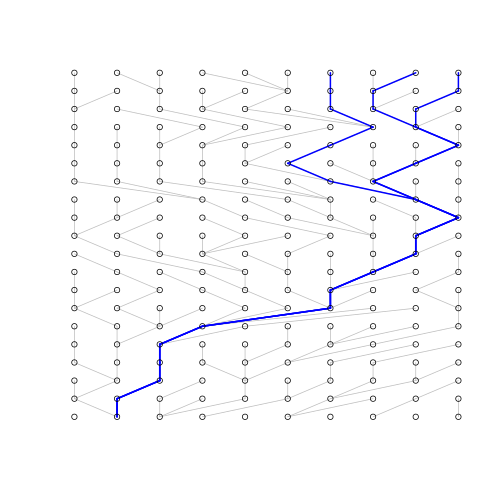
\includegraphics[scale=0.5]{CreateFisherWrightExample}

\caption{Wright-Fisher model. The circles represent haploid individuals of
multiple generation. Each (horizontal) generation consists of ten
individuals. In this example there are twenty generations, going from
the current time (top) into the past (bottom). The grey lines show
the inheritance of genes from parents to offspring.\label{fig:Wright-Fisher-model}}
\end{figure}


The simulation model used in figure \ref{fig:Wright-Fisher-model}
is a Wright-Fisher model (also depicted in figure \ref{fig:Wright-Fisher-model})
that follows the inheritance of an allele in a constant-size population
of individuals. Due to stochasticity, not all parents will be chosen
to have surviving offspring, as some parents will have more than one.
This implies that, out of the initial population, given enough time,
only one common ancestor has given rise to all lineages in the present.
Thus, when going back in time following a subset of lineages, these
lineages will coalesce into their direct ancestors, eventually ending
up in the common ancestor of all lineages. 

A CPCM has many convenient mathematical properties. As an example,
I will show how to calculate the likelihood of a simple phylogeny,
as depicted in figure \ref{fig:ExamplePhylogenyCoalescent}, that
has three branches in the present time $T$. Three branches means
two branching times, which are $ts=\{t_{2},t_{3}\}=\{4,3\}$.  Note
that this is only the phylogeny of the individuals sampled, and that
the total population size (or species pool) is much larger than the
sample size.

\begin{figure}[H]
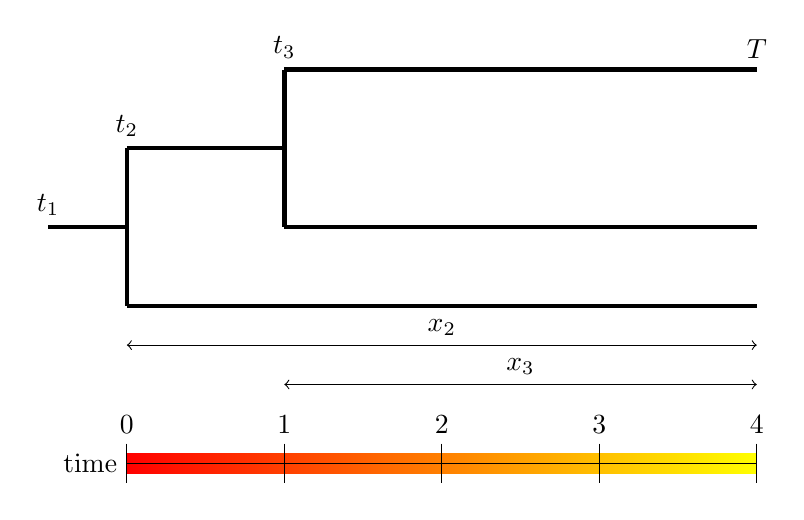
\begin{tikzpicture} 
  \draw[ultra thick] (-1, 0) node[anchor=south] {$t_1$}  -- (0, 0) node {}; 
  \draw[ultra thick] ( 0, 1) node[anchor=south] {$t_2$}  -- (2, 1) node {}; 
  \draw[ultra thick] ( 0, 1) node               {     }  -- (0,-1) node {}; 
  \draw[ultra thick] ( 0,-1) node               {     }  -- (8,-1) node {}; 
  \draw[ultra thick] ( 2, 2) node[anchor=south] {$t_3$}  -- (8, 2) node[anchor=south] {$T$}; 
  \draw[ultra thick] ( 2, 2) node               {     }  -- (2, 0) node {}; 
  \draw[ultra thick] ( 2, 0) node               {     }  -- (8, 0) node {}; 
  % xs
  \draw[<->] (0, -1.5) node {} -- (4, -1.5) node[anchor=south] {$x_2$} -- (8,-1.5) node {}; 
  \draw[<->] (2, -2.0) node {} -- (5, -2.0) node[anchor=south] {$x_3$} -- (8,-2.0) node {}; 
  % Bars underneath
  \shade[left color=red,right color=yellow] (0,-3-0.125) rectangle (8,-3+0.125);
  \draw (0, -3) node[anchor=east] {time}  -- (8, -3) node {}; 
  \draw (0, -2.75) node[anchor=south] {$0$}  -- (0, -3.25) node {}; 
  \draw (2, -2.75) node[anchor=south] {$1$}  -- (2, -3.25) node {}; 
  \draw (4, -2.75) node[anchor=south] {$2$}  -- (4, -3.25) node {}; 
  \draw (6, -2.75) node[anchor=south] {$3$}  -- (6, -3.25) node {}; 
  \draw (8, -2.75) node[anchor=south] {$4$}  -- (8, -3.25) node {}; 
\end{tikzpicture}

\caption{Example phylogeny showing the relation between time (setting crown
age at time zero), branching times ($ts$) and branch lengths ($xs$)
\label{fig:ExamplePhylogenyCoalescent}}
\end{figure}


\[
\mathcal{L}(N,ts)=\prod_{i=2}^{n}\left[\frac{1}{N}\left(\begin{array}{c}
i\\
2
\end{array}\right)e^{-\left(\begin{array}{c}
i\\
2
\end{array}\right)\frac{t_{i}}{N}}\right]
\]


\begin{equation}
\mathcal{L}(N,ts=\{t_{2},t_{3}\}=\{4,3\})=\left[\frac{1}{N}\left(\begin{array}{c}
2\\
2
\end{array}\right)e^{-\left(\begin{array}{c}
2\\
2
\end{array}\right)\frac{4}{N}}\right]\left[\frac{1}{N}\left(\begin{array}{c}
3\\
2
\end{array}\right)e^{-\left(\begin{array}{c}
3\\
2
\end{array}\right)\frac{3}{N}}\right]\label{eq:LikelihoodCPCM}
\end{equation}


From this likelihood, multiple population sizes can be suggested and
have their likelihoods calculated. Figure \ref{fig:LikelihoodsCPCM}
shows the likelihood for different values of $N$. From that same
figure, we can conclude that the most likely population size is $N=7$.

\begin{figure}
\includegraphics[scale=0.4]{LikelihoodCoalescent}

\caption{Constant-size coalescent model likelihoods plotted for different population
sizes $N$. It can be observed that $N=7$ has the highest likelihood\label{fig:LikelihoodsCPCM}}
\end{figure}


Within this research, this model is used to estimate a constant species
diversity. Within this context, it is reasonable to use the same assumptions
as in haploid populations, as new species are created from one single
species.

A constant-sized individual-based model is assumed to yield similar
phylogenies as a constant-size coalescent model, when the IBM satisfies
the conditions to allow for using coalescence.


\subsection{Time-dependent speciation\label{sub:Time-dependent-speciation}}

Just for completion I mention the time-dependent birth-death models,
in which the speciation rate changes with time. This is a family of
models, because the function that calculates the speciation rate in
time can be of any shape. Time-dependent speciation models assume
that speciation rate is caused by an external force. Examples of these
external forces are climate change and/or the mass extinction event
due to humans. The likelihood has been derived \cite{harvey1994phylogenies}.


\subsection{Diversity-dependent speciation\label{sub:Density-dependent-model}}

According to the fossil record, species diversity reaches a certain
limit (e.g. \cite{alroy2010shifting}). The exact mechanism, how current
species diversity affects speciation, is still unknown. One mechanism
is niche-filling (e.g. \cite{schluter2009evidence}), which states
that the number of niches is limited, thus allowing only for a limited
number of species (note that the argument can also be turned around,
where species create niches\cite{odling2003niche}. 

Whatever the mechanism, a diversity-dependent model lets the number
of species present inhibit its increase. The expected number of lineages
through time is not a simple equation anymore, and can be found in
\cite{etienne2011diversity}. Figure \ref{fig:EtienneEtAl2012Fig1c},
however, shows the outcome.

\begin{figure}
\includegraphics[scale=0.5]{EtienneEtAl2012Fig1c}

\caption{Lineages-through-time plot in a diversity-dependent model for crown
age 15 Myr for different extinction rates $\mu$. The speciation rate
$\lambda_{0}$ is set to 0.8 $Myr^{-1}$ (this is the speciation rate
without diversity dependence lowering the observed speciation rate)
. The number of lineages expected at equilibrium, $K$, is set to
40. From \cite{etienne2011diversity}\label{fig:EtienneEtAl2012Fig1c}}
\end{figure}


Diversity-dependent speciation model (with extinction) yields a better
match with molecular phylogenies than other models \cite{etienne2011diversity}
(as can be observed in figure \ref{fig:EtienneEtAl2012Fig2ab}).

\begin{figure}
\includegraphics[scale=0.25]{EtienneEtAl2012Fig2}

\caption{Fit of diversity-dependent model to phylogenetic data. Data from the
left picture, the foraminifera, is based on fossils \cite{aze2011phylogeny}.
Data from the right picture, the cetaceans, is based on a molecular
phylogeny calibrated with fossils \cite{steeman2009radiation}. The
lines denotes the best of a diversity-dependent model with (green)
and without (light red) extinction. From \cite{etienne2011diversity}\label{fig:EtienneEtAl2012Fig2ab}}
\end{figure}



\subsection{Protracted speciation\label{sub:Protracted-speciation}}

Protracted speciation provides an alternative mechanism to the unknown
mechanism of diversity-dependent (instantaneous) speciation \cite{etienne2012prolonging}.
Pivotal to the protracted speciation model is the assumption that
speciation takes time. The protracted speciation model is an extension
of the birth-death model: when the speciation time is set to zero,
the protracted speciation model reduces to a birth-death model. The
approximate likelihood of a protracted speciation model has been derived
recently \cite{lambert2015reconstructed}. 

An expression for the expected number of lineages through time has
been derived \cite{etienne2012prolonging}. Figure \ref{fig:EtienneRosindell2012Fig2}
shows the expected number of lineages through time for a protracted
pure-birth model, whereas figure \ref{fig:EtienneRosindell2012Fig4}
shows this for a protracted birth-death model.

\begin{figure}
\includegraphics[scale=0.3]{EtienneRosindell2012Fig2}

\caption{Lineages-through-time plot in a pure-birth protracted speciation model,
for speciation initiation rate $\lambda_{1}=0.5$. From \cite{etienne2012prolonging}\label{fig:EtienneRosindell2012Fig2}}
\end{figure}


\begin{figure}
\includegraphics[scale=0.3]{EtienneRosindell2012Fig4}

\caption{Lineages-through-time plot in a protracted birth-death model, for
different extinction rates ($\mu_{1}$and $\mu_{2}$) and different
speciation completion rate $\lambda_{2}$. speciation initiation rate
$\lambda_{1}$ is set to $0.5$ in all plots. From \cite{etienne2012prolonging}\label{fig:EtienneRosindell2012Fig4}}
\end{figure}


The protracted speciation model is illustrated with some good fits
to the molecular phylogenies \cite{etienne2012prolonging}, as shown
in figure \ref{fig:EtienneRosindell2012Fig6}.

\begin{figure}
\includegraphics[scale=0.25]{EtienneRosindell2012Fig6}

\caption{LTT plots of four bird phylogenies (the dots) and their fits (the
lines) to a protracted speciation model. The number of lineages through
time was derived from molecular data \cite{phillimore2008density}.
The grey line is the best fit of a protracted pure-birth model using
maximum likelihood. The black line is the best fit of a protracted
birth-death model using a least-squares method. Picture from \cite{etienne2012prolonging}\label{fig:EtienneRosindell2012Fig6}}
\end{figure}


Note that the fit of a birth-death protracted model in figure \ref{fig:EtienneRosindell2012Fig6}
is done by a least-squares method as there was no likelihood equation
available at that time. 

The keen observer sees that the LTT plots to illustrate the protracted
speciation model (figure \ref{fig:EtienneRosindell2012Fig6}, using
the dataset from \cite{phillimore2008density}) would also fit well
to a diversity-dependent model (LTT plots shown in figure \ref{fig:EtienneEtAl2012Fig1c},
using the dataset from \cite{aze2011phylogeny}), but this model comparison
has not been performed. It would be appropriate to fit both models
to the other data set as well. Will molecular phylogenies be able
to conclude a clear winner of the two suggested null models? This
leads me to suggest the research project described at chapter \ref{sub:RQ4:influence-tree-prior}.


\subsection{Age-dependent speciation\label{sub:Age-dependent-speciation}}

A recent model, the age-dependent model, assumes that speciation rates
are dependent on the age of the lineage \cite{hagen2015age}. It is
closely related to the protracted speciation model, but outcompetes
it in producing phylogenies with the $\beta$ statistic (a measure
of tree imbalance) as found in nature. The median $\beta$ statistic
in emperical trees has a value of $-1$ \cite{aldous1996probability}.
The protracted speciation model produces many phylogenies with the
same value of $\beta$, but the distribution around this value is
very wide. This in contrast to the age-dependent speciation model,
which provides phylogenies with the value of $\beta$ found in nature
with less variance. The critique warrants a deeper comparison between
these two potential future null models. This leads me to suggest the
research project described in chapter \ref{sub:RQ3:compare-lineage-diversification-models}.


\section{Comparing models\label{sec:Comparing-models}}

How to select the best model? And what exactly do we mean by 'best'?
This is already an old, but still important question. Anscombe's Quartet,
published in 1972, \cite{anscombe1973graphs} (figure \ref{fig:Anscombe's-Quartet})
is a nice example of the equally good fit of a linear model to several
very different data sets, with (close to) equal mean and variance
in terms of sum of error squared. When looking at the data, however,
the fit looses its sensibility. Anscombe argues we should always visualize
the data, instead of fitting a line or curve through it blindly \cite{anscombe1973graphs}. 

\begin{figure}
\includegraphics[scale=0.25]{AnscombesQuartet}

\caption{Anscombe's Quartet. All four data sets have (close to) equal mean
and variance. The line is fit to the data by lowest sum of errors
squared, which is (approximately) equal for all data sets. The top-left
plot shows a satisfactory fit, where the others give a more satisfactory
fit by using a quadratic curve or remove an outlier\cite{anscombe1973graphs}\label{fig:Anscombe's-Quartet}}
\end{figure}


In this research, it is the other way around: it is about selecting
the model behind the data. And there is ample literature on model
selection (e.g. \cite{burnham2002model,wit2012all}). In this context,
'What is the best model?' has two meanings (after \cite{wit2012all}):
(1) which modelling procedure will, with sufficient data, identify
the true model? and (2) based on the data, which model lies closest
to the true model? Unsurprisingly, there are many ways to compare
models, each comparison having its own pros and cons: Akaike Information
Criterion, Bayes Factor, Bayesian Information Criterion, Deviance
Information Criterion, false discovery rate, Focused Information Criterion,
likelihood-ratio test, Mallows $C_{p}$, minimum description length,
posterior-predictive tests, Widely Applicable Information Criterion,
not naming close derivatives such as $AIC_{c}$ of members of this
incomplete list \cite{wit2012all,green1995reversible,nylander2005model}. 

The most important frequentist test is the Akaike Information Criterion
(AIC, as discussed in chapter \ref{sub:Akaike-Information-Criterion}),
the most important Bayesian test is the Bayesian Information Criterion
(BIC). For the frequentist approach, I will describe the common hierarchical
likelihood-ratio test (hLRT) and the AIC, for the Bayesian approach
I will describe the Bayes Factor and BIC. Note that \cite{posada2004model}
has a nice comparison of the hLRT, Bayes Factor and AIC.

These techniques can yield the best model, but this may not be an
adequate model. This can be tested by penelized likelihood, parametric
bootstrap and posterior predictive checks \cite{nylander2005model}. 


\subsection{Hierarchical likelihood-ratio test\label{sub:Hierarchical-likelihood-ratio-test}}

The frequentist's toolbox is commonly equipped with the hierarchical
likelihood-ratio test (hLRT) \cite{posada2004model}. An hLRT can
be used for models that have a known maximum likelihood function and
are nested. 

Suppose we have a model that serves as a null hypothesis $H_{0}$
and a more elaborate model $H_{1}$ that may or may not fit the observed
data significantly better. The models must be nested: it must be possible
that a certain parameter combination of $H_{1}$ reduces it to $H_{0}$
. For example, an Ornstein-Uhlenbeck process can be reduced to a Brownian
motion by setting its mean reversion rate to zero. Let the parameters
fitting the null model best (as found by maximum likelihood) be $\hat{\theta_{0}}$,
where $\hat{\theta_{1}}$ are the best parameters for the alternative
model, on the same observed data $X$. The test statistic $\Delta$
is then defined as \cite{posada2004model,salemi2003phylogenetic,nylander2005model}:

\begin{equation}
\Delta=2\left(\mathcal{L}(\hat{\theta_{1}}\mid X)-\mathcal{L}(\hat{\theta_{0}}\mid X)\right)\label{eq:LikelihoodRatioTest}
\end{equation}


$\mathcal{L}(\theta{}_{i}\mid X)$ is the maximized log likelihood
of (the parameters of) model $i$ given the data $X$. $\Delta$,
called the deviance, follows approximately a $\chi^{2}$ distribution.
This distribution has as many degrees of freedom as the alternative
model has more parameters than the null model. If the LRT is located
in the rejection area of the $\chi^{2}$ distribution the null hypothesis
is rejected and the alternative model is said to have a significantly
higher likelihood.

\begin{figure}
\includegraphics[scale=0.4]{CppQwtExample11}

\caption{Probability density function of a $\chi^{2}$ distribution for different
degrees of freedom}
\end{figure}


\begin{figure}
\includegraphics[scale=0.25]{ToolStochasticityInspector_reject_H0}

\caption{StochasticityInspector correctly rejecting an Ornstein-Uhlenbeck process
being a Brownian motion, for a signicance level of $\alpha=0.05$.
The degrees of freedom is 2, as an Ornstein-Uhlenbeck process has
two additional parameters (the mean reversion rate and a target mean),
resulting in a critical p-value of 5.991465. The value of delta at
the bottom right is the same as $\Delta$ in equation \ref{eq:LikelihoodRatioTest}}
\end{figure}


It is argued that the hLRT is not the best candidate in comparing
phylogenetic models for multiple reasons. For instance, the hLRT assumes
that at least one of the models is true (as otherwise the test statistic
does not follow a $\chi^{2}$ distribution anymore \cite{kent1982robust}),
where the AIC and Bayes factor do allow model uncertainty \cite{posada2004model}.
For a more elaborate comparison, see \cite{posada2004model}.


\subsection{Akaike Information Criterion\label{sub:Akaike-Information-Criterion}}

The most commonly used tool to compare models by the frequentist is
the Akaike Information Criterion (AIC). Every model has an AIC dependent
on the $k$ number of parameters it has and a maximum log likelihood
of $\mathcal{L}(\hat{\theta_{0}}\mid X)$ as shown by equation \ref{eq:AIC}
(from \cite{posada2004model,nylander2005model,lemey2009phylogenetic}):

\begin{equation}
AIC=2k-2\mathcal{L}(\hat{\theta}\mid X)\label{eq:AIC}
\end{equation}


The preferred model is the model with the lowest AIC. The first term,
$2k$, has a $2$ to correct for asymptotic bias (thus the $2$ is
not arbitrary at all). In a phylogenetic context, $k$ may also include
an estimated tree topology. If this is so, then twice the number of
taxa minus three mujst be added to $k$\cite{lemey2009phylogenetic}.
The second term, $2\mathcal{L}(\hat{\theta}\mid X)$, also has a $2$
with the function of making the entire term asymptotically chi-squared
\cite{burnham2002model}. The AIC assumes a large sample size. If
the sample size is small, the closely related $AIC_{c}$ can take
the sample size into account.

AICs can also be compared by their weights, where the AIC weight of
model $i$ is defined as:

\[
W_{AIC_{i}}=e^{-\frac{1}{2}AIC_{i}}
\]


Then the chance $p$, that the model with AIC score $AIC_{i}$ is
correct, equals: 

\begin{equation}
p\left(AIC_{i}\right)=\frac{W_{AIC_{i}}}{\sum\left(W_{AIC}\right)}\label{eq:AIC_model_probability}
\end{equation}



\subsection{Bayes factors\label{sub:Bayes-factors}}

Bayes factors can be viewed as the Bayesian analog of an LRT (the
latter being described in chapter \ref{sub:Hierarchical-likelihood-ratio-test}).
The Bayes factor $B_{ij}$ of two models, $M_{i}$ and $M_{j}$ equals
the ratio between the model posteriors $Pr(D\mid M_{i})$ and $P(D\mid M_{j})$
that use parameters $\theta_{i}$ with data $D$.

\begin{equation}
B_{ij}=\frac{Pr(D\mid M_{i})}{Pr(D\mid M_{j})}=\frac{\intop Pr\left(\theta_{1}\mid M_{1}\right)Pr\left(D\mid\theta_{1},M_{1}\right)d\theta_{1}}{\intop Pr\left(\theta_{2}\mid M_{2}\right)Pr\left(D\mid\theta_{2},M_{2}\right)d\theta_{2}}\label{eq:BayesFactor}
\end{equation}


A model's posterior $Pr$ is the integral of the likelihoods over
all parameters weighted by the prior, as opposed to maximum likelihood.
The interpretation of values of $B_{ij}$ is given in table \ref{tab:Interpretation-of-Bayes-Factor}.

\begin{table}
\begin{tabular}{|c|c|}
\hline 
Condition & Interpretation\tabularnewline
\hline 
\hline 
$B_{ij}>150$ & Evidence for $M_{i}$ very strong\tabularnewline
\hline 
$12<B_{ij}<150$ & Evidence for $M_{i}$ strong\tabularnewline
\hline 
$3<B_{ij}<12$ & Evidence for $M_{i}$ positive\tabularnewline
\hline 
$1<B_{ij}<3$ & Evidence for $M_{i}$ barely worth mentioning\tabularnewline
\hline 
$B_{ij}<1$ & Negative support for $M_{i}$\tabularnewline
\hline 
\end{tabular}

\caption{Interpretation of Bayes factor $B_{ij}$ when comparing models $M_{i}$
and $M_{j}$ , after \cite{raftery1996hypothesis,nylander2005model,posada2004model}.
\label{tab:Interpretation-of-Bayes-Factor}}
\end{table}


Drawback of using Bayes factors is that they are difficult to compute. 


\subsection{Bayesian Information Criterion\label{sub:Bayesian-Information-Criterion}}

The Bayesian Information Criterion (BIC) is an information criterion
closely related to the AIC (see chapter \ref{sub:Akaike-Information-Criterion}).
The preferred model is the model with the lowest BIC. A model $\mathcal{M}$
has a BIC dependent on maximum log-likelihood $l\left(\hat{\theta}\right)$(where
$\hat{\theta}$ are the parameters yielding the maximum likelihood)
for a parameter space of $p$ dimensions and sample size of $n$,
as shown in equation (from \cite{wit2012all}):

\begin{equation}
BIC(\mathcal{M})=2l\left(\hat{\theta}\right)+p\cdot ln(n)\label{eq:BIC}
\end{equation}


Note that in phylogenetics, the sample size is an open area for research
\cite{nylander2005model}. Choosing the lowest BIC is one way to
select a best model, a more Bayesian approach will be to compare model
weights $W(\mathcal{M})$ of all models in the following fashion \cite{wit2012all,burnham2004multimodel}:

\[
W\left(\mathcal{M}\right)=e^{-\frac{1}{2}BIC(\mathcal{M})}
\]


\begin{equation}
p\left(\mathcal{M}_{0}\mid y\right)=\frac{W(\mathcal{M}{}_{0})}{\sum\left(W(\mathcal{M})\right)}\label{eq:Posterior_model_probability}
\end{equation}


The posterior model probability $p\left(\mathcal{M}_{i}\mid y\right)$
of model $\mathcal{M}_{i}$ gives the probability the model is correct
in making future predictions.


\subsection{Hastie and Green's reversible-jump MCMC}

This paragraph is a brief mention of a very interesting idea by Hastie
and Green \cite{hastie2012model}: instead of pitting competing models
against each other (each samples with their own MCMC), let a single
MCMC sample run through the different models, occasionally jumping
between models. In 1995 already, it was shown that this is fundamentally
possible \cite{green1995reversible}, yet there still are many difficulties
to overcome \cite{wit2012all}. In phylogentics, BAMM is an example
that can switch between multiple time- and diversity-dependent speciation
models \cite{rabosky2014automatic}. 


\section{Trait stochasticity\label{sec:Trait-stochasticity}}

Imagine a species having a trait, and that trait value changing in
time. The trait value is changed by recombination and mutation, two
processes with a stochastic property. A trait value in time will be
different with or without selection, thus there are already two types
of stochastic processes. A neutral trait can be modeled as a Brownian
motion, which is an undirected random process. It is the ancestor
of all other stochastic processes and discussed in chapter \ref{sub:Brownian-Motion}.
Traits that are non-neutral and have an optimum value can be modeled
by an Ornstein-Uhlenbeck process, which modifies the Brownian motion
by adding a certain target mean to converge to. Because of its general
use, it is discussed in chapter \ref{sub:Ornstein-Uhlenbeck}. There
are also other models I will only briefly mention here:
\begin{itemize}
\item A single-burst (SB) model assumes that the mean of a Brownian motion
can have a major shift once \cite{uyeda2011million}, for example
when an adaptive radiation takes place
\item A multiple-burst (MB) model is an Brownian motion that can have multiple
major shifts \cite{uyeda2011million}, for example when adaptive radiations
takes place. Close to this is the punctuated equilibrium (PE) model
which assumes that most trait fluctuations take place at speciation.
There is some controversy around PE, as Pennell et al argue that the
PE model tries to capture multiple conceptually distinct ideas (evolution
being pulsed or gradual, most trait evolution occurring during radiation
or not) in a single framework \cite{pennell2014there}.
\end{itemize}
It is important to understand the process governing a trait value
in time. A trait value following a Brownian motion is neutral, thus
has no biological forces acting on it. Detecting the stochastic process
underlying noisy data increases our focus on investigating traits
that have a larger biological relevance.


\subsection{Brownian Motion\label{sub:Brownian-Motion}}

A Brownian motion (BM) model is described by the Wiener process, a
continuous-time stochastic process. A Wiener process has changes that
are independent and drawn from a normal distribution with mean zero
and constant variance. This results in an expected mean of zero. An
example of a Brownian motion described by James Brown in 1827 is the
motion of a pollen grain through water. The stochastic differential
equation for the BM model is:

\begin{equation}
dx_{t}=\sigma dW_{t}\label{eq:BM-SDE}
\end{equation}


The value changing in time is denoted $x$ by rate $dx_{t}$. The
only term is a noise term, where $\sigma$ is the volatility or noise
strength and $W_{t}$ is a Wiener process. The exact solution of this
SDE is given by equation \ref{eq:BM-recurrent}:

\begin{equation}
x_{t+\delta}=x_{i}+\sigma\sqrt{\delta}N_{0,1}\label{eq:BM-recurrent}
\end{equation}


Equation \ref{eq:BM-recurrent} is a recurrence equation that calculates
the value of $x$ at time $t+\Delta$ from the current value of $x$
at timepoint $t$. The equation allows for a sampling time $\delta$,
which is positive and can be less than $1$. An example run is shown
in figure \ref{fig:Example-Brownian-motion-run}.

\begin{figure}
\includegraphics[scale=0.35]{BrownianMotionRun}

\caption{Example Brownian motion run. The parameters can be seen at the left:
the run length is set to $t=100$ for volatility $\sigma=\frac{1}{2}$.
The initial value of $x$ is set to zero. At the right, the values
generated by the run are used to recover the parameters, where the
estimated volatility $\hat{\sigma}\approx0.37$. The difference between
$\sigma$ and $\hat{\sigma}$ is caused by stochasticity. StochasticityInspector
(\protect\url{www.richelbilderbeek.nl/ToolStochasticityInspector.htm})
is used for visualisation\label{fig:Example-Brownian-motion-run}}
\end{figure}


The log-likelihood function of a BM model is known, given the set
of observations $X=\left\{ x_{0},x_{1},\ldots,x_{n}\right\} $:

\begin{equation}
\mathcal{L}(X,\sigma^{2})=-\frac{n}{2}\cdot ln\left(2\pi\sigma^{2}\right)-\sum_{i=1}^{n}\frac{\left(x_{i}-x_{i-1}\right)^{2}}{2\cdot\sigma^{2}}\label{eq:LogLikelihoodBm}
\end{equation}


where the maximum likelihood estimator is:

\begin{equation}
\hat{\sigma^{2}}=\frac{1}{n}\sum_{i=1}^{n}\left(x_{i}-x_{i-1}\right)^{2}\label{eq:MaxLikelihoodVolatilityBm}
\end{equation}


The estimated volatility $\hat{\sigma}$ is the maximum likelihood
estimates given the set of observations $X$. The estimated parameters
will differ from the true known parameters (to generate the data),
which is caused by the random noise of the Wiener process.


\subsection{Ornstein-Uhlenbeck\label{sub:Ornstein-Uhlenbeck}}

An Ornstein-Uhlenbeck (OU) model is a stochastic process that is attracted
to a mean value and it is a member of the single stationary peak (SSP)
models \cite{harmon2010early}. An example OU process is a particle
under Brownian motion experiencing friction. The stochastic differential
equation for the OE model is:

\begin{equation}
dx_{t}=\theta\left(\mu-x_{t}\right)dt+\sigma dW_{t}\label{eq:OU-SDE}
\end{equation}


The value changing in time is denoted $x$ by rate $dx_{t}$. Value
$x$ is attracted to long-term mean $\mu$. The difference between
$x$ and $\mu$ sets the direction of the slope of the SDE, which
allows $x$ to decrease its distance to $\mu$. The strength $x$
converges to $\mu$ is determined by the mean reversion rate $\theta$,
where $\theta>0$. The first term would could $x$ to converge to
$\mu$ with a speed of $\theta$. The second term is a noise term,
where $\sigma$ is the volatility or noise strength and $W_{t}$ is
a Wiener process. Note that a Wiener process is a synonym for Brownian
motion.

The exact solution of this SDE is given by equation \ref{eq:OU-recurrence}:

\begin{equation}
x_{t+1}=x_{i}e^{-\theta\delta}+\theta\left(1-e^{-\theta\delta}\right)+\sigma\sqrt{\frac{1-e^{-2\theta\delta}}{2\theta}}N_{0,1}\label{eq:OU-recurrence}
\end{equation}


Equation \ref{eq:OU-recurrence} is a recurrence equation that calculates
the value of $x$ at time $t+\delta$ from the current value of $x$
at timepoint $t$. The equation allows for a sampling time, $\delta$,
which can be less than $1$. An example run is shown in figure \ref{fig:Example-Ornstein-Uhlenbeck-run}.

\begin{figure}
\includegraphics[scale=0.4]{OrnsteinUhlenbeckWithLikelihood}

\caption{Example Ornstein-Uhlenbeck run. The parameters can be seen at the
left: the run length is set to $t=100$ for long-term mean $\mu=1$,
mean reversion rate $\theta=1$, volatility $\sigma=\frac{1}{2}$
and sampling frequency $\delta=1$. The initial value of $x$ is set
to zero and can be seen to converge to the long-term mean. At the
right, the values generated by the run are used to recover the parameters.
Note that the estimates are close to, but not exactly the same as
the parameters used to simulate the data. This is caused by stochasticity
and a finite sampling time. StochasticityInspector (\protect\url{www.richelbilderbeek.nl/ToolStochasticityInspector.htm})
is used for visualisation\label{fig:Example-Ornstein-Uhlenbeck-run}}
\end{figure}


The log-likelihood function of an OU model is known, given the set
of observations $X=\left\{ x_{0},x_{1},..,x_{n}\right\} $:

\[
\alpha=\sigma^{2}\cdot\frac{1-e^{-2\theta\delta}}{2\theta}
\]


\begin{equation}
\mathcal{L}(X,\delta,\theta,\mu,\sigma)=-\frac{n}{2}\cdot ln\left(2\pi\right)-n\cdot ln(\alpha)-\frac{1}{2\alpha^{2}}\sum_{i=1}^{n}\left[x_{i}-x_{i-1}e^{-\theta\delta}-\mu\left(1-e^{-\theta\delta}\right)\right]^{2}\label{eq:LogLikelihoodOu}
\end{equation}


The value of $\alpha$ is just a constant used to simplify the notation.
A negative value of $\theta$ denotes repulsion. For $\theta=0$,
the likelihood equation of a Brownian motion must be used (equation
\ref{eq:LogLikelihoodBm}), to prevent a division by zero. There exists
a unique point in which all partial derivatives are zero, which allows
to estimate the maximum likelihood of all variables. To calculated
the maximum likelihood estimates $\hat{\theta}$, $\hat{\mu}$ and
$\hat{\sigma}$ given the set of observations $X$ and sampling time
$\delta$, the convenient constants $S_{x}$,$S_{y}$,$S_{xx}$,$S_{xy}$,$S_{yy}$,$\alpha$
and $\beta$ are used: 

\[
S_{x}=\sum_{i=1}^{n}x_{i-1}
\]


\[
S_{y}=\sum_{i=1}^{n}x_{i}
\]


\[
S_{xx}=\sum_{i=1}^{n}x_{i-1}^{2}
\]


\[
S_{xy}=\sum_{i=1}^{n}x_{i-1}x_{i}
\]


\[
S_{yy}=\sum_{i=1}^{n}x_{i}^{2}
\]


\begin{equation}
\hat{\mu}=\frac{S_{y}S_{xx}-S_{x}S_{xy}}{n\left(S_{xx}-S_{xy}\right)-\left(S_{x}^{2}-S_{x}S_{y}\right)}\label{eq:OU-est-target-mean}
\end{equation}


\begin{equation}
\hat{\theta}=-\frac{1}{\delta}\cdot ln\left(\frac{S_{xy}-\hat{\mu}S_{x}-\hat{\mu}S_{y}+n\left(\hat{\mu}{}^{2}\right)}{S_{xx}-2\hat{\mu}S_{x}+n\left(\hat{\mu}{}^{2}\right)}\right)\label{eq:OU-est-mean-reversion-rate}
\end{equation}


\[
\alpha=e^{-\hat{\theta}\delta}
\]


\[
\beta=\frac{1}{n}\left[S_{yy}-2\alpha S_{xy}+\alpha^{2}S_{xx}-2\hat{\mu}\left(1-\alpha\right)\left(S_{y}-\alpha S_{x}\right)+n\left(\hat{\mu}{}^{2}\right)\left(1-\alpha\right)^{2}\right]
\]


\begin{equation}
\hat{\sigma}=\sqrt{\beta\frac{2\theta}{1-\alpha^{2}}}\label{eq:OU-est-volatility}
\end{equation}


The estimated parameters will differ from the true known parameters
(to generate the data), which is caused by the random noise of the
Wiener process and the finite size of the sample. A worked example
can be found in chapter \ref{sub:Worked-example-OU}.


\subsection{Early burst}

An Early Burst (EB) model is a member of the accelerate/decelarate
(ACDC) process family. EB can be implemented as a Brownian motion
with a time-dependent dispersion parameter, where the trait $x$ follows
this recurrence equation \cite{blomberg2003testing}:

\[
x_{t+1}=x_{t}+\gamma(t)
\]


where $\gamma(t)$ is a noise term, with the variance $V$ of this
noise being dependent on the standard deviation of the noise $\sigma_{\gamma}$
(at time $t=0$) and change rate $g$ which determines if noise increases
($g>1$) or decreases ($g<1$) in time as:

\[
V\left(\gamma\left(t\right)\right)=\sigma_{\gamma}^{2}\cdot g^{-t}
\]



\section{Individual-based modeling\label{sec:IBM-modeling}}

One of the modeling techniques closest to nature is individual-based
modeling. IBMs are so common, that there are at least 38 toolkits
to generate them (Nikolai \& Madey (2009)). One of the models important
to this research is the Unified Neutral Theory of Biodiversity model
(Hubbell, 2001). This is an influential individual-based model that
assumes individuals from different species may be modeled equivalently. 


\subsection{UTEM model\label{sub:UTEM-model}}

The Unified Theory of Ecology and Macroevolution model \cite{rosindell2015unifying}
is an extension that allows for mild selection. This UTEM model follows
a Moran structure (a constant number of lineages and overlapping generations)
and is spatially implicit. Every lineage has a competitive trait,
which increases its probability in reproduction. 

\begin{figure}
\includegraphics[scale=0.4]{RosindellEtAl2015Fig1}

\caption{One timestep in the UTEM model. First, an individual is randomly chosen
to die. Then an individual is chosen to reproduce, where individuals
with a higher competitive trait (depicted as the number in the circles)
have a higher probability of being chosen. This offspring has either
an identical, higher or lower competitive trait, with these probabilities
being dependent on mutation rate $\mu$. Note that although this picture
suggests a spatial structure, in the currently available model this
is absent. Picture from \cite{rosindell2015unifying}\label{fig:RosindellEtAl2015Fig1}}
\end{figure}


As expected, this costless trait will increase indefinitely (see figure
\ref{fig:RosindellEtAl2015Screenshot3D} for a 3D visualisation). 

\begin{figure}
\includegraphics[scale=0.5]{RosindellEtAl2015}

\caption{Visualisation of competitive traits in time. Time goes from left to
right. Initialially, all lineages have the same competitive trait
value. Trait values go from front to back (away from the camera),
but this is difficult to observe from this point of view. The number
of different traits is stacked. From \protect\url{https://github.com/richelbilderbeek/RosindellEtAl2015}\label{fig:RosindellEtAl2015Screenshot3D}}
\end{figure}


When allowing for speciation to take time, this model results in realistic
phylogenies similar to those in the protracted speciation model. This
model is an interesting new approach with aspects of both ecology
and evolutionary biology. It would be interesting if the model would
also produce realistic spatial patterns, that is why I suggest it
as a research project in chapter \ref{sub:RQ2:Spatial-patterns}.

But there might be something more interesting to be discoved in the
model: a to-be-added additional neutral trait at the individual level
may not follow a Brownian walk in its trait value anymore at the species
level. Would this be the case, this will cast older predictions in
doubt (similar philosophy as by \cite{pigot2015new}) that draw conclusions
from a trait deviating from the assumed null hypothesis, which is
currently assumed to be a Brownian motion. Checking if this null hypothesis
is correct is an important topic and suggested as a research project
in chapter \ref{sub:RQ1:Trait-fluctuations-species-level}.


\section{Coalescent modeling\label{sec:Coalescent-modeling}}

Some IBMs qualify for a shortcut. As an example, when modeling a Fisher-Wright
simulation in an individual-based way, many redundant calculations
will be performed. For example, in figure \ref{fig:Redundance-in-individual-based-modeling},
only three individuals are sampled, where the many individuals encircled
have had no effect on this sample. 

\begin{figure}
\includegraphics[scale=0.25]{IbmNotNeeded}

\caption{Redundance in individual-based modeling: three individuals have been
sampled in the present (top) and their coalescence tree is constructed.
The individuals encircled have had no influence on the sampled individuals\label{fig:Redundance-in-individual-based-modeling}}
\end{figure}


Coalescent modeling can only been done under the condition that interactions
are time-reversible. If this condition is satisfied, algorithms based
on coalescence techniques can be multiple orders of magnitude faster
(the algorithm is described in chapter \ref{sub:Coalescence-simulation-algorithm}).
This speed increase is achieved because only the individuals sampled
are tracked back in time, because lineages that were to go extinct
are not created and because the simulation starts at (the vital) equilibrium
conditions. Reaching equilibrium conditions is important (it is there
where the analytical calculations meet the simulation), and common
IBMs cannot detect when having reached equilibrium. IBMs just run
longer than needed to be (more) sure the equilibrium is reached. 


\subsection{Coalescence simulation algorithm\label{sub:Coalescence-simulation-algorithm}}

A coalescence simulation algorith first creates a coalescent tree,
then puts speciation events on this tree, after which it can conclude
a phylogeny. A good introductory paper of this technique in a spatial
context is \cite{rosindell2008coalescence}. Generations can both
be overlapping and seperated and both will have the same equilibrium
distribution, although the dynamics to reach it will be different
\cite{etienne2007neutral}.

The coalescent technique has been benchmarked and compared to a regular
IBM in estimating species richness in a spatial context, where it
had a 36000 fold speed improvement over a regular IBM\cite{rosindell2008coalescence}.
Figure \ref{fig:Rosindell2008EtAl_3D} shows a 3D visualisation of
that spatial model's lineages going back in time.

\begin{figure}
\includegraphics[scale=0.4]{RosindellEtAl2008_3D}

\caption{Visualization of the coalescent technique in a spatial model. In the
present (bottom) 3x3 lineages are sampled. Going back in time (up)
one needs to keep track of fewer and fewer lineages due to coalescence
of these lineages. Simulation from Rosindell et al., 2008, 3D visualization
by RJCB (code can be downloaded from \protect\url{https://github.com/richelbilderbeek/ProjectRichelBilderbeek})\label{fig:Rosindell2008EtAl_3D}}
\end{figure}



\section{Monte Carlo Markov Chain\label{sec:MCMC}}

A Monte Carlo Markov Chain (MCMC) is a technique to obtain a representative
sample of a huge parameter state space. It will result in a sequence
('Chain') of draws from a distribution. When traversing this chain,
only that current position matters, rendering it a Markov chain. 'Monte
Carlo' (known for its casino) is a metaphor of randomness being involved
in going to a next state in the chain. 

In this section, we are interested in finding a combination of a phylogeny
and parameters. Here I discuss how to obtain a representative sample
of a phylogeny and parameter set combinations, using Bayes' theorem
to move through the chain. Bayes' theorem is described at chapter
\ref{sub:Bayes'-theorem}. How Bayes' theorem is used to navigate
through parameter space is described in chapter \ref{sub:Searching-through-parameter-space}.
The drawback of using an MCMC is described in chapter \ref{sub:Drawbacks-of-Bayesian-joint-inference}.


\subsection{Bayes' theorem\label{sub:Bayes'-theorem}}

What is the probability a hypothesis is true, given the evidence observed?
Bayes' theorem paves the way to rationally estimate this probability.
Bayes' theorem is known in multiple forms, one shown as equation \ref{eq:BayesTheorem}.
where $P$ denotes a probability, $H$ denotes a hypothesis and $E$
denotes evidence:

\begin{equation}
P(H\mid E)=\frac{P(E\mid H)P(H)}{P(E)}\label{eq:BayesTheorem}
\end{equation}


To estimate this probability, one needs to know the likelihood, $P(E\mid H)$,
which is the probability the evidence is observed if the hypothesis
is true. The likelihood is weighted by the prior, $P(H)$, which is
the probability the hypothesis is true without any evidence. The third
term, the marginal likelihood, $P(E)$, is (1) the most difficult
to calculate, and (2) of least importance. The marginal likelihood
ensures that the sum of all hypothesis-evidence combinations sums
up to 100\%. 

The result of this equation is called the posterior, $P(H\mid E)$,
and it corresponds to the updated belief in the hypothesis. This belief
is updated, because the prior hypothesis did not take the evidence
into account. Note that the posterior can be re-used as the next prior,
resembling a belief that is changed by evidence.

Bayes' theorem can be applied in many areas of research, including
this research, where it is used to fit a species tree model to molecular
data.


\subsection{Example}
\begin{quote}
Elvis Presley had a twin brother who died at birth. What is the probability
that Elvis had an identical twin? (from MacKay, 2003). Assume 8\%
of all twins are monozygous.
\end{quote}
This question gives more insight than at first glance.

Let us assume the hypothesis $H$ that Elvis had an identical twin
(given that he had a twin brother). The prior probability this hypothesis
is true, $P(H)$, is 8\%. If the brother is monozygous, the likelihood,
$P(E\mid H)$, of observing a male sibling is 100\%. The probability
of observing a male sibling, $P(E)$, is (1) the probability of observing
a male sibling if monozygous (which is 100\%) multiplied by (2) the
probability of observing a male sibling if dizygotic (which is 50\%)

\[
P(H\mid E)=\frac{P(E\mid H)P(H)}{P(E)}=\frac{100\%\cdot8\%}{50\%}=16\%
\]


At first glance one might miss the information that Elvis' sibling
was a male, although it is easy to see that the probability Elvis
would have a monozygous sister is zero.


\subsection{Navigate through parameter space\label{sub:Searching-through-parameter-space}}

The size of the parameter space to is huge. For just the phylogeny,
equation \ref{eq:Number-of-phylogenies} shows how the number of possible
phylogenies skyrockets by increasing the number of taxa. Using MCMC
one can obtain a representative sample of phylogenies and parameters,
where the most likely combination of phylogeny and parameters are
represented more often.

Before doing this, already some assumptions have to be stated about
the system: what likelihood function (and thus model) is used, which
parameters are jointly inferred and which priors are used. A prior
is what you believe before seeing the data. For example, a birth-rate
cannot be zero, nor negative, but is unlikely to be infinitely large
as well. This information can be specified explicity for the MCMC.
The simplest prior is a flat prior, which assumes a certain range
to be possible and another range to be impossible. It is, however,
not advised to use flat priors, as the MCMC will reach equilibrium
slower. A better prior for a birth-death rate may be a gamma distribution.
It is good to specify close-to-flat piors as these will hardly affect
the result of the MCMC but it does give a direction to process, allowing
it to reach equilibrium faster.

Let us define a state as the combination of a certain phylogeny and
parameters. For example, assuming a pure-birth model, our state has
the tree structure $((A:0.3,B:0.3):0.7,(C:0.6,D:0.6):0.4);$ (as shown
in figure \ref{fig:example_phylogeny}) and birth rate $\lambda=1.0$.
The log-likelihood of this state is approximately $3.0$ . The entire
parameter space is filled with states such as these with a certain
spatial structure. Our focal state is, for example, connected to a
state with the same phylogeny but a slightly different birth rate.
Additionally, it may be connected to a state with the same birth rate,
but with a slightly different phylogeny. 

\begin{figure}
\includegraphics[scale=0.25]{ExamplePhylogeny}

\caption{Depiction of the example phylogeny $((A:0.3,B:0.3):0.7,(C:0.6,D:0.6):0.4);$\label{fig:example_phylogeny}}
\end{figure}


Any two states are connected by an operator. There are operators working
on the birth rate and on the phylogeny. An example operator working
on birth rate can be a change in its value sampled from a normal distribution
of mean zero and small standard deviation. An example operator on
the phylogeny may be a change in edge length(s) or a swap of two taxa.

Operators are weighted by a Hastings factor, which is a correction
that allows for a symmetric state search; that is: it might be that
going from state A to B is easier than the other way around. The Hastings
factor corrects for this. From every state, with a weighed probability,
an operator to follow is selected randomly.

When having arrived at a new state, the likelihood of this new state
is determined. If it has a higher likelihood, this new state is always
accepted as the starting point for the next iteration. If the new
state has a lower likelihood, the probability of accepting this state
is proportional of the ratio of the likelihoods of the current and
new state. This decision algorithm is called the Metropolis-Hastings
algorithm.

It may be that the initial state was unrepresentative of the parameter
space. For a huge parameter space as in this research, this is even
extremely likely. To obtain a representative sample of parameter space,
one lets the MCMC reach the representative parameter space first.
This is called the burn-in of the MCMC. The samples drawn before burn-in
are discarded. 

When the MCMC is in the representative part of parameter space, the
sampling process can start. Not all samples are used, because two
subsequent samples are highly correlated. To obtain uncorrelated samples
one takes a sample every, say, one thousand steps. These samples are
representative of the full parameter space and are called (a sample
from) the posterior distribution. The posterior distribution is often
saved to a file for further analysis.


\subsection{Drawbacks of MCMC\label{sub:Drawbacks-of-Bayesian-joint-inference}}

MCMC is time-intensive and can take multiple days on a computer cluster,
especially when flat priors are used. Additionally, it may be that
instead of a representative parameter space, the MCMC gets stuck in
a local pocket of high likelihoods. One trick to get the MCMC escape
this pocket is to use heated priors (heated priors were named after
wax, which is much softer when heated).

BEAST2 (an abbreviation of 'Bayesian Evolutionary Analysis by Sampling
Trees') is a tool to do Bayesian inference on phylogenies. See chapter
\ref{sec:BEAST2} for more detail.


\section{BEAST\label{sec:BEAST2}}

BEAST2 ('Bayesian Evolutionary Analysis by Sampling Trees') is a tool
to do Bayesian joint-inference \cite{drummond2015bayesian}(Bayesian
joint-inference is described in chapter \ref{sec:MCMC}). It creates
a posterior distribution (consisting of phylogeny and parameter estimates)
from molecular alignments.

BEAST2 is the successor of BEAST, differing mostly in the software
architecture. BEAST and BEAST2 are developed in the obligate object-oriented
language Java. BEAST2 facilites extensions of the program by use of
class inheritance, which is visualized by ModelBuilder (see figure
\ref{fig:ModelBuilder}).

\begin{figure}[H]
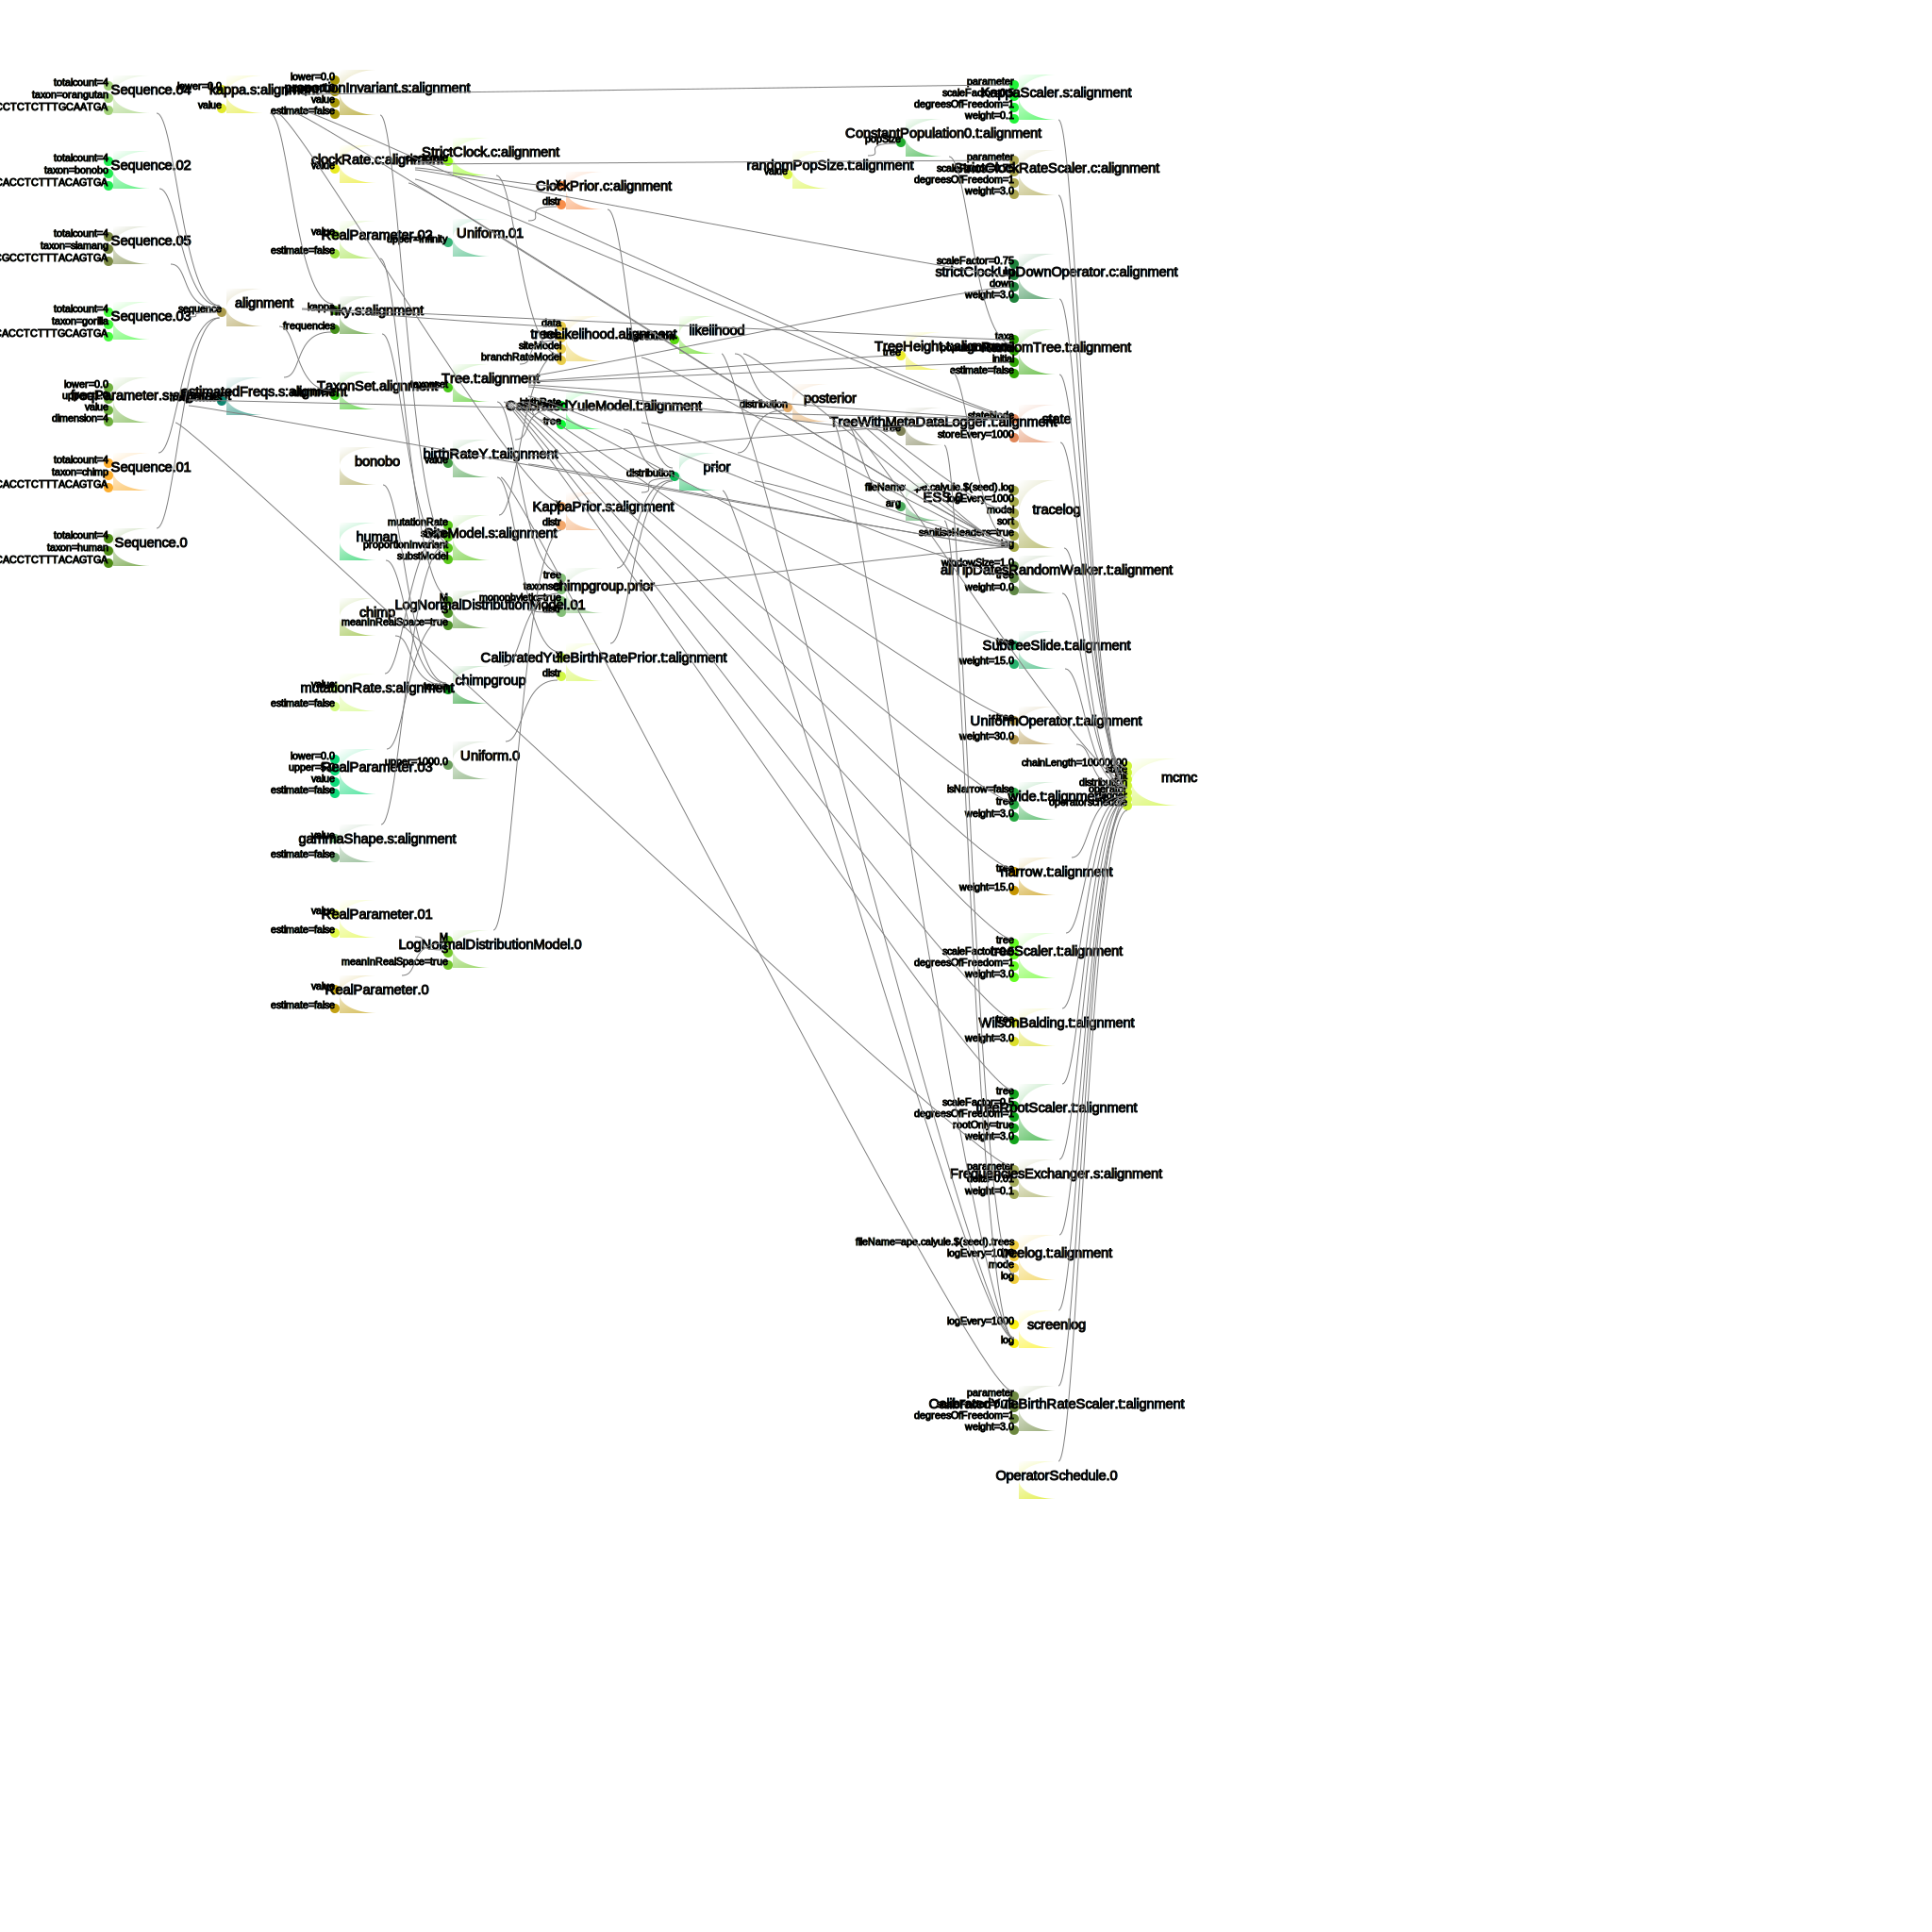
\includegraphics[scale=0.2]{ModelBuilderExample}

\caption{ModelBuilder, a tool supplied with BEAST2 that shows the modular architecture
of BEAST2\label{fig:ModelBuilder}}
\end{figure}


BEAST2 is accompanied by other tools, among others:
\begin{itemize}
\item Beauti (Bayesian Evolutionary Analysis Utility): to create a parameter
file
\item DensiTree: draw trees
\item FigTree: draw trees
\item Tracer: to analyse the posterior
\end{itemize}
The first step to use BEAST2, is to create a BEAST2 input  file using
Beauti (see chapter \ref{sub:Beauti:Create-Beast2-parameter-file}).
With this input file, BEAST2 generates a posterior distribution (see
chapter \ref{sub:BEAST2:Running-BEAST2}). The posterior distribution
is checked for convergence with Tracer (see chapter \ref{sub:BEAST2:Checking-with-TRACER}).
If the posterior has converged, it is analyzed (see chapter \ref{sub:BEAST2:Analysing-the-results}).


\subsection{Beauti\label{sub:Beauti:Create-Beast2-parameter-file}}

BEAST2 uses an XML file as input. Beauti ensures these input files
are created in a user-friendly and correct way. The latter is accomplished
by only displaying those models and priors relevant to the current
situation. For example, it will only suggest DNA nucleotide substitution
models if the molecular alignment is of DNA type. Note that this research
starts with DNA alignments, where it has been shown that different
unaligned sequences result in different phylogenies \cite{wong2008alignment}.
Additionally, the genes are assumed to be identical by descent (aka
orthologs). 

\begin{figure}[H]
\includegraphics[scale=0.5]{BeautiPriors}

\caption{Beauti: priors\label{fig:Beauti:tree-priors}}
\end{figure}


The tree priors (see figure \ref{fig:Beauti:tree-priors}) embody
different speciation models and thus are the most interesting in this
research. Here I will describe the tree priors I consider most relevant
:
\begin{itemize}
\item Yule: corresponds to the (diversity independent) pure-birth model
described in chapter \ref{sub:Yule-model}. This model is the simplest
to use as it has the fewest parameters. This model is adviced to use
if the data consists of DNA sequences that have one individual per
species\cite{drummond2015bayesian}
\item Birth-death model: this (diversity-independent) model is described
in chapter \ref{sub:Birth-death-model}. In BEAST2, the birth-death
model is advised to be used only if all extant species are present
in the dataset. If some are missing, an additional variable should
be added, which resembles the proportion of extant species sampled
\cite{yang1997bayesian,stadler2009incomplete}
\item Constant population size coalencent: this model is described in chapter
\ref{sub:Constant-size-coalescent-model} for lineages in a species
pool (instead of individuals in a population)
\item Exponential population size coalescent: described in chapter \ref{sub:Exponential-growth-coalescent-model}
\end{itemize}
Note that not all models I have described are available in BEAST2.
It will be the by-product of some research projects to add these.
For example, the research project described in chapter \ref{sub:Project-DD-vs-protracted}
needs a tool to do Bayesian analysis of the protracted speciation
model. This may not be as easy as adding the known likelihood, as
BEAST2 assumes that species are monophyletic, whereas in protracted
speciation this may not always be the case. It is known that in BEAST2,
if the clade is not monophyletic, the MCMC chain may mix poorly \cite{drummond2015bayesian},
but the extent of this problem in the desired context is unknown.


\subsection{Running BEAST2\label{sub:BEAST2:Running-BEAST2}}

\begin{figure}[H]
\includegraphics[scale=0.5]{Beast}

\caption{BEAST2 running\label{fig:BEAST2-running}}
\end{figure}


BEAST2 is started from the command-line and needs the parameter filename
as an argument (see figure \ref{fig:BEAST2-running} for a screenshot).
Every certain number of timesteps, it shows the last used parameter
candidates, with their likelihoods. The output is written to multiple
files.


\subsection{Checking with TRACER\label{sub:BEAST2:Checking-with-TRACER}}

\begin{figure}[H]
\includegraphics[scale=0.5]{Tracer}

\caption{Tracer\label{fig:Tracer}}
\end{figure}


BEAST2 creates multiple files as output. Tracer can be used to conveniently
check the result for convergence:
\begin{itemize}
\item The burn-in should have removed onset effects
\item All effective sample sizes (which relates to the confidence of the
posterior being sampled adequately) should be at least 100. Values
of 700-800 are very good, but values beyond 1000 are unnecessary high
\cite{drummond2015bayesian}
\item All variables in the posterior should have a smooth distribution
\end{itemize}

\subsection{Analysing the results\label{sub:BEAST2:Analysing-the-results}}

\begin{figure}[H]
\includegraphics[scale=0.33]{DensiTreeExample}

\caption{DensiTree showing a concensus tree\label{fig:DensiTree-showing-a-consensus-tree}}
\end{figure}


DensiTree can be used to view a concensus tree (see figure \ref{fig:DensiTree-showing-a-consensus-tree}).
Additionally, the file containing the posterior (as a text file) can
be easily analyzed with, for example, the R programming language.


\section{Research questions}


\subsection{Research question 1: Will neutral traits behave Brownian in an individual-based
model on different species-levels?\label{sub:RQ1:Trait-fluctuations-species-level}}

Neutral traits follow a Brownian motion at the level of the individual.
However, most studies assume that trait values follow Brownian motion
at the species level. And this assumption is also extended to the
clade level. Because analytical methods rely on this assumed normal
distribution of traits at the species level, one may wonder whether
this causes a bias if the traits actually evolve via Brownian motion
at the individual level. The null hypothesis is that neutral traits
behave as a Brownian motion on all levels. This null hypothesis is
first tested in a simple non-spatial model, a spatial model and the
UTEM model (see chapter \ref{sub:UTEM-model}). If this null hypothesis
is incorrect, older conclusions will need to be revised.


\subsection{What is the influence of the tree prior on Bayesian estimation of
the phylogeny?\label{sub:RQ4:influence-tree-prior}}

When using a Bayesian approach, one credo often used is 'Let the data
speak for itself'. This is based on the idea that a prior gets less
and less relevant with an increasing amount of data. This project
intends to see how much this is the case for the tree prior used in
Bayesian phylogenetics. As a dataset simulated phylogenies will be
used. Next to using the existing BEAST2 tree priors, also a new prior,
the protracted speciation model, will be added, as this would be the
first model in BEAST2 that does not assume instanteous speciation.

The models that will be used are:
\begin{itemize}
\item Exponential-population coalescent model
\item Constant-population birth-death model
\item Constant rate birth-death model
\item Protracted speciation model
\end{itemize}
The most interesting contrasts will be the constant rate birth-death
versus the exponential-population coalescent (see chapter \ref{sub:Birth-death-model}).
It is important to know how well the Bayesian approach can select
the right model with the highest probability: if we cannot clearly
infer the process from simulated data, we will be powerless on real
data. Questions that will be answered are:
\begin{itemize}
\item What is the model power: given a phylogeny constructed with model
A, what is its power of explaining the data compared with other models? 
\item How good are the models at recovering their own parameters?
\end{itemize}

\subsection{What are the predicted macro-ecological and macro-evolutionary patterns
of a spatially explicit version of UTEM?\label{sub:RQ2:Spatial-patterns}}

The protracted speciation model has already shown a good fit to molecular
phylogenies in spatially implicit models. Already since the inception
of the protracted speciation model in 2010 (Rosindell et al., 2010)
it has been suggested to investigate the phylogenies generated in
a spatial model. This suggestion is warranted as it might be that
the realistic phylogenies created are artifacts of the unrealistic
assumptions of the spatially implicit model. This project will investigate
if the protracted speciation model will still result in realistic
phylogenies by adding a spatial structure to the model. Would the
protracted speciation model still hold or should others be preferred
as a better null model?

This question will be extended to the UTEM model (see chapter \ref{sub:UTEM-model}),
which is -as the authors already acknowledge- biologically unrealistic,
due to lack of spatiality. Would spatiality be built into the model,
will the model break down, or still provide us with an alternative
mechanism to produce realistic phylogenies? And will it still produce
the macro-ecological and macro-evolutionary patterns as in the orignal
model? What will the patterns in the ecology and evolutionary traits
be?


\subsection{How distinct are current models predicting a slow-down in lineage
diversification?\label{sub:RQ3:compare-lineage-diversification-models}}

Although currently the birth-death and coalescent models are heavily
used, development of more realistic models is ongoing. Because it
is observed that there is a limit to the maximum number of species,
multiple mechanisms have been suggested to realize this behavior:
\begin{itemize}
\item The current species diversity has an effect on speciation rate, which
is the assumption underlying diversity-dependent speciation as discussed
in chapter \ref{sub:Density-dependent-model}
\item Speciation takes time, which is the assumption of the protracted speciation
model as discussed in chapter \ref{sub:Protracted-speciation}
\item Speciation rates decrease by branch length, which is the age-specific
model as described in chapter \ref{sub:Age-dependent-speciation}
\end{itemize}
It is important to know the contrast of these models before facing
real data, as it will be troublesome if these models do not give a
clear signal on simulated data. Questions that will be answered are:
\begin{itemize}
\item What is the model power: given a phylogeny constructed with model
A, how often will A be recognized as yielding the best fit? 
\item What is the type I error of each model: given a phylogeny constructed
with model A, how often will A be rejected as being the model that
generated the phylogeny?
\item How good are the models at recovering their own parameters?
\end{itemize}



\section{Planning}


\subsection{Main activities}



\begin{table}[H]
\begin{tabular}{|c|c|c|c|}
\hline 
 & Start, first day of & First draft, first day of & End, last day of\tabularnewline
\hline 
\hline 
RQ 1 & May 2015 & March 2016 & May 2016\tabularnewline
\hline 
RQ 2 & June 2016 & April 2017 & Aug 2017\tabularnewline
\hline 
RQ 3 & Sep 2017 & Feb 2018 & May 2018\tabularnewline
\hline 
RQ 4 & June 2018 & Nov 2018 & Jan 2019\tabularnewline
\hline 
Thesis & Feb 2019 & June 2019 & Aug 2019\tabularnewline
\hline 
\end{tabular}

\caption{Planning}
\end{table}


\begin{figure}[H]
\includegraphics[scale=0.5]{Planning}

\caption{Planning}
\end{figure}



\subsection{Other repeated activities}
\begin{itemize}
\item April: assist Community Ecology Research
\item October: assist in Evolutionary Ecology Research 
\item October: assist in Ecological Interactions
\end{itemize}

\subsection{Other singular activities}
\begin{itemize}
\item 2015-07-08: MMEE conference
\item 2015-08-??: Go/NoGo meeting
\item 2015-09-??: presentation BEAST
\end{itemize}

\section{Acknowledgements}

C�sar Martinez was hulpful in deriving the likelihood equations \ref{eq:Likelihood-BD}
and \ref{eq:LikelihoodCPCM}. Thanks to Ana Depetris for suggesting
helpful improvements on parts of an early draft of this manuscript.


\section{Worked examples}

To allow the reader to check his/her calculations, I supply these
worked examples.


\subsection{Worked example Brownian motion\label{sub:Worked-example-BM}}

The values of $x$ in time $t$ for a volatility $\sigma$ can be
calculated from numbers drawn from a random distribution with mean
zero and standard deviation zero $N_{0,1}$ as in equation \ref{eq:BM-recurrent}.

\[
x_{t+1}=x_{i}+\sigma N_{0,1}
\]


See table \ref{tab:BM} how a the values following a Brownian motion
are calculated from random numbers.

\begin{table}
\begin{tabular}{|c|c|c|}
\hline 
$t$ & $x$ & $N_{0,1}$\tabularnewline
\hline 
\hline 
0 & 0 & -\tabularnewline
\hline 
1 & 0.607535 & 1.21507\tabularnewline
\hline 
2 & 0.726817 & 0.238564\tabularnewline
\hline 
3 & 0.596934 & -0.259766\tabularnewline
\hline 
4 & 0.830478 & 0.467088\tabularnewline
\hline 
5 & 0.734508 & -0.191939\tabularnewline
\hline 
6 & 0.380306 & -0.708404\tabularnewline
\hline 
7 & 0.62205 & 0.483487\tabularnewline
\hline 
8 & -0.0411321 & -1.32636\tabularnewline
\hline 
9 & 0.666996 & 1.41626\tabularnewline
\hline 
10 & 0.603708 & -0.126575\tabularnewline
\hline 
\end{tabular}

\caption{Brownian motion values $x$ in time $t$ for volatility $\sigma=0.5$
and initial $x=0$. The random numbers $N_{0,1}$drawn follow a normal
distribution with mean zero and standard deviation one. To calculate
$x_{i}$, the $N_{0,1}$in that row is used. Due to this, there is
no random value in the first row, as no random value was used in calculating
$t_{0}$. The random numbers are generated by the Mersenne Twister
pseudo random-number generator as described in \cite{matsumoto1998mersenne}
and implemented in the C++14 Standard std::mersenne\_twister\_engine
class \cite{becker2011working} seeded with the value 83\label{tab:BM}}
\end{table}



\subsection{Worked example Brownian motion max likelihood parameter estimation}

In this worked example, I use the Brownian motion as in chapter \ref{sub:Worked-example-BM}.
Equation \ref{eq:MaxLikelihoodVolatilityBm} shows how to calculate
the volatility estimated to have the highest likelihood $\hat{\sigma^{2}}$,
where we already know that $n=11$. Table \ref{tab:BM-likelihood-sum-term}
shows the terms in that equation, resulting in:

\[
\hat{\sigma^{2}}=\frac{1}{n}\sum_{i=1}^{n}\left(x_{i}-x_{i-1}\right)^{2}=\frac{1}{11}\cdot1.5931101=0.1448282
\]


\[
\hat{\sigma}=\sqrt{\hat{\sigma}^{2}}=0.3805630
\]


\begin{table}
\begin{tabular}{|c|c|c|}
\hline 
$t$ & $x$ & Term\tabularnewline
\hline 
\hline 
0 & 0 & -\tabularnewline
\hline 
1 & 0.607535 & 0.3690988\tabularnewline
\hline 
2 & 0.726817 & 0.0142282\tabularnewline
\hline 
3 & 0.596934 & 0.0168696\tabularnewline
\hline 
4 & 0.830478 & 0.0545428\tabularnewline
\hline 
5 & 0.734508 & 0.0092102\tabularnewline
\hline 
6 & 0.380306 & 0.1254591\tabularnewline
\hline 
7 & 0.62205 & 0.0584402\tabularnewline
\hline 
8 & -0.0411321 & 0.4398105\tabularnewline
\hline 
9 & 0.666996 & 0.5014454\tabularnewline
\hline 
10 & 0.603708 & 0.0040054\tabularnewline
\hline 
\hline 
$\sum$ & 5.7281999 & 1.5931101\tabularnewline
\hline 
\end{tabular}

\caption{Calculating the sum term in equation \ref{eq:MaxLikelihoodVolatilityBm}
from the Brownian motion as in table \ref{tab:BM}\label{tab:BM-likelihood-sum-term}}
\end{table}


Calculating the maximum log-likelihood, following equation \ref{eq:LogLikelihoodBm}
(note that $\sigma^{2}$cannot be replaced by $\sigma$):

\[
\mathcal{L}(X,\sigma^{2}=\hat{\sigma^{2}})=-\frac{n}{2}\cdot ln\left(2\pi\sigma^{2}\right)-\sum_{i=1}^{n}\frac{\left(x_{i}-x_{i-1}\right)^{2}}{2\cdot\sigma^{2}}=-4.9811847
\]


\begin{table}
\begin{tabular}{|c|c|c|}
\hline 
$t$ & $x$ & Term\tabularnewline
\hline 
\hline 
0 & 0 & \tabularnewline
\hline 
1 & 0.607535 & 1.2742643\tabularnewline
\hline 
2 & 0.726817 & 0.0491209\tabularnewline
\hline 
3 & 0.596934 & 0.0582400\tabularnewline
\hline 
4 & 0.830478 & 0.1883017\tabularnewline
\hline 
5 & 0.734508 & 0.0317971\tabularnewline
\hline 
6 & 0.380306 & 0.4331306\tabularnewline
\hline 
7 & 0.62205 & 0.2017569\tabularnewline
\hline 
8 & -0.0411321 & 1.5183870\tabularnewline
\hline 
9 & 0.666996 & 1.7311733\tabularnewline
\hline 
10 & 0.603708 & 0.0138280\tabularnewline
\hline 
\hline 
$\sum$ & 5.7281999 & 5.5\tabularnewline
\hline 
\end{tabular}

\caption{Calculating the sum term in equation \ref{eq:MaxLikelihoodVolatilityBm}
from the Brownian motion as in table \ref{tab:BM} and a known estimated
volatility $\hat{\sigma}=0.3805630$\label{tab:BM-likelihood-sum-term-1}}
\end{table}



\subsection{Worked example Ornstein-Uhlenbeck maximum likelihood\label{sub:Worked-example-OU}}

In this example we use a Brownian motion (with volatility of 0.5,
as worked out in chapter \ref{sub:Worked-example-BM}) to estimate
all Ornstein-Uhlenbeck parameters. From those, the maximum log-likelihood
is calculated. Table \ref{tab:Worked-example-OU} shows the values
of $x$ and the calculation of all summation terms.

\begin{table}
\begin{tabular}{|c|c|c|c|c|c|c|}
\hline 
$t$ & $x$ & $S_{x}$ & $S_{y}$ & $S_{xx}$ & $S_{xy}$ & $S_{yy}$\tabularnewline
\hline 
\hline 
0  & 0  & 0 & - & - & - & -\tabularnewline
\hline 
1 & 0.607535  & 0.607535 & 0.607535 & 0 & 0 & 0.3690988\tabularnewline
\hline 
2 & 0.726817  & 0.726817 & 0.726817 & 0.3690988 & 0.4415695 & 0.5282630\tabularnewline
\hline 
3 & 0.596934  & 0.596934 & 0.596934 & 0.5282630 & 0.4338618 & 0.3563302\tabularnewline
\hline 
4 & 0.830478  & 0.830478 & 0.830478 & 0.3563302 & 0.4957406 & 0.6896937\tabularnewline
\hline 
5 & 0.734508  & 0.734508 & 0.734508 & 0.6896937 & 0.6099927 & 0.5395020\tabularnewline
\hline 
6 & 0.380306  & 0.380306 & 0.380306 & 0.5395020 & 0.2793378 & 0.1446327\tabularnewline
\hline 
7 & 0.62205  & 0.62205 & 0.62205 & 0.1446327 & 0.2365694 & 0.3869462\tabularnewline
\hline 
8 & -0.0411321  & -0.0411321 & -0.0411321 & 0.3869462 & -0.0255862 & 0.0016918\tabularnewline
\hline 
9 & 0.666996  & 0.666996 & 0.666996 & 0.0016918 & -0.0274349 & 0.4448837\tabularnewline
\hline 
10 & 0.603708 & - & 0.603708 & 0.4448837 & 0.4026708 & 0.3644633\tabularnewline
\hline 
\hline 
$\sum$ & 5.7281999 & 5.1244919 & 5.7281999 & 3.4610420 & 2.8467186 & 3.8255054\tabularnewline
\hline 
\end{tabular}

\caption{Example data for the worked example of the Ornstein-Uhlenbeck max
likelihood estimations\label{tab:Worked-example-OU}}
\end{table}


Because the timepoints go from $t=0$ to (and including) $t=10$ in
steps of 1 time unit, $n=11$ and $\delta=1$. Now filling in equations
\ref{eq:OU-est-target-mean} to \ref{eq:OU-est-volatility}:

\[
\hat{\mu}=\frac{S_{y}S_{xx}-S_{x}S_{xy}}{n\left(S_{xx}-S_{xy}\right)-\left(S_{x}^{2}-S_{x}S_{y}\right)}=0.5316637
\]


\[
\hat{\theta}=-\frac{1}{\delta}\cdot ln\left(\frac{S_{xy}-\hat{\mu}S_{x}-\hat{\mu}S_{y}+n\left(\hat{\mu}{}^{2}\right)}{S_{xx}-2\hat{\mu}S_{x}+n\left(\hat{\mu}{}^{2}\right)}\right)=1.7961973
\]


\[
\alpha=e^{-\hat{\theta}\delta}=0.1659287
\]


\[
\beta=\frac{1}{n}\left[S_{yy}-2\alpha S_{xy}+\alpha^{2}S_{xx}-2\hat{\mu}\left(1-\alpha\right)\left(S_{y}-\alpha S_{x}\right)+n\left(\hat{\mu}{}^{2}\right)\left(1-\alpha\right)^{2}\right]=0.0739099
\]


\[
\hat{\sigma}=\sqrt{\beta\frac{2\theta}{1-\alpha^{2}}}=0.5225234
\]


Filling in these values in equation \ref{eq:LogLikelihoodOu} results
in the maximum log-likelihood:

\[
\alpha^{2}=\sigma^{2}\cdot\frac{1-e^{-2\theta\delta}}{2\theta}=0.0739099
\]


\[
\mathcal{L}(X,\delta,\theta,\mu,\sigma)=-\frac{n}{2}\cdot ln\left(2\pi\right)-n\cdot ln(\alpha)-\frac{1}{2\alpha^{2}}\sum_{i=1}^{n}\left[x_{i}-x_{i-1}e^{-\theta\delta}-\mu\left(1-e^{-\theta\delta}\right)\right]^{2}
\]


\[
\mathcal{L}(X,\delta=1,\theta=\hat{\theta},\mu=\hat{\mu},\sigma=\hat{\sigma})=0.0489702
\]


\begin{table}
\begin{tabular}{|c|c|c|}
\hline 
$t$ & $x$ & Term\tabularnewline
\hline 
\hline 
0 & 0 & \tabularnewline
\hline 
1 & 0.607535 & 0.02692538\tabularnewline
\hline 
2 & 0.726817 & 0.03332964\tabularnewline
\hline 
3 & 0.596934 & 0.00108167\tabularnewline
\hline 
4 & 0.830478 & 0.08293483\tabularnewline
\hline 
5 & 0.734508 & 0.02348938\tabularnewline
\hline 
6 & 0.380306 & 0.03423069\tabularnewline
\hline 
7 & 0.62205 & 0.01334045\tabularnewline
\hline 
8 & -0.0411321 & 0.34550117\tabularnewline
\hline 
9 & 0.666996 & 0.05307289\tabularnewline
\hline 
10 & 0.603708 & 0.00245905\tabularnewline
\hline 
\hline 
$\sum$ & 5.7281999 & 0.61636516\tabularnewline
\hline 
\end{tabular}

\caption{Calculating the sum term in equation \ref{eq:LogLikelihoodOu} from
the Ornstein Uhlenbeck process as in table \ref{tab:Worked-example-OU},
using $\delta=1$, target mean $\mu=0.5316637$, mean reversion rate
$\theta=1.7961973$ and a volatility $\sigma=0.5225234$\label{tab:OU-likelihood-sum-term}}
\end{table}



\subsection{Worked example hLRT between Brownian motion and Ornstein Uhlenbeck}

For this worked example, we will apply the hierarchical likelihood-ratio
test (note that the (non-log) likelihoods must be used, see equation
\ref{eq:LikelihoodRatioTest}) on the maximum log-likelihood of the
Brownian motion $\mathcal{L}_{BM}(X,\sigma^{2}=\hat{\sigma^{2}})$
(calculated in chapter \ref{sub:Worked-example-BM}) and the maximum
log-likelihood of the Ornstein-Uhlenbeck process $\mathcal{L}_{OU}(X,\delta=1,\theta=\hat{\theta},\mu=\hat{\mu},\sigma=\hat{\sigma})$
(calculated in chapter \ref{sub:Worked-example-OU}). Both (log)likelihoods
have been calculated from the same dataset (see chapter \ref{sub:Worked-example-BM}),
so they can be compared. Additionally, the Brownian motion process
is a simpler model than Ornstein-Uhlenbeck, so putting all equations
into place:

\[
\mathcal{L}_{BM}(X,\sigma^{2}=\hat{\sigma^{2}})=-4.9811847
\]


\[
\mathcal{L}_{OU}(X,\delta=1,\theta=\hat{\theta},\mu=\hat{\mu},\sigma=\hat{\sigma})=0.0489702
\]


\[
\Delta=2\left(\mathcal{L}(\hat{\theta_{1}}\mid X)-\mathcal{L}(\hat{\theta_{0}}\mid X)\right)=2\left(\mathcal{L}_{OU}(X,\delta=1,\theta=\hat{\theta},\mu=\hat{\mu},\sigma=\hat{\sigma})-\mathcal{L}_{BM}(X,\sigma^{2}=\hat{\sigma^{2}})\right)=10,060309702669839
\]


The critical $P_{critical}$ value for significance level $\alpha=0.05$
and degrees of freedom $dof=2$ (the alternative model, OU, has 2
more parameters than the null model, BM) 

\[
P_{critical}=\chi^{2}(\alpha=0.05,dof=2)=5.991465
\]


The null hypothesis is that the data is generated by the null model,
which is Brownian motion. Would $\Delta<P_{critical}$ then the null
hypothesis cannot be rejected. In this example, however, $\Delta>P_{critical}$,
so there is enough statistical evidence to reject the null model.

\bibliographystyle{plain}
\bibliography{IntroductoryEssay}

\begin{lyxcode}
\end{lyxcode}

\end{document}
